\documentclass[]{article}
\usepackage{lmodern}
\usepackage{amssymb,amsmath}
\usepackage{ifxetex,ifluatex}
\usepackage{fixltx2e} % provides \textsubscript
\ifnum 0\ifxetex 1\fi\ifluatex 1\fi=0 % if pdftex
  \usepackage[T1]{fontenc}
  \usepackage[utf8]{inputenc}
\else % if luatex or xelatex
  \ifxetex
    \usepackage{mathspec}
  \else
    \usepackage{fontspec}
  \fi
  \defaultfontfeatures{Ligatures=TeX,Scale=MatchLowercase}
\fi
% use upquote if available, for straight quotes in verbatim environments
\IfFileExists{upquote.sty}{\usepackage{upquote}}{}
% use microtype if available
\IfFileExists{microtype.sty}{%
\usepackage{microtype}
\UseMicrotypeSet[protrusion]{basicmath} % disable protrusion for tt fonts
}{}
\usepackage[margin=1in]{geometry}
\usepackage{hyperref}
\hypersetup{unicode=true,
            pdftitle={Surface Detection by Robot Movements - Report},
            pdfauthor={Marian Dumitrascu},
            pdfborder={0 0 0},
            breaklinks=true}
\urlstyle{same}  % don't use monospace font for urls
\usepackage{color}
\usepackage{fancyvrb}
\newcommand{\VerbBar}{|}
\newcommand{\VERB}{\Verb[commandchars=\\\{\}]}
\DefineVerbatimEnvironment{Highlighting}{Verbatim}{commandchars=\\\{\}}
% Add ',fontsize=\small' for more characters per line
\usepackage{framed}
\definecolor{shadecolor}{RGB}{248,248,248}
\newenvironment{Shaded}{\begin{snugshade}}{\end{snugshade}}
\newcommand{\AlertTok}[1]{\textcolor[rgb]{0.94,0.16,0.16}{#1}}
\newcommand{\AnnotationTok}[1]{\textcolor[rgb]{0.56,0.35,0.01}{\textbf{\textit{#1}}}}
\newcommand{\AttributeTok}[1]{\textcolor[rgb]{0.77,0.63,0.00}{#1}}
\newcommand{\BaseNTok}[1]{\textcolor[rgb]{0.00,0.00,0.81}{#1}}
\newcommand{\BuiltInTok}[1]{#1}
\newcommand{\CharTok}[1]{\textcolor[rgb]{0.31,0.60,0.02}{#1}}
\newcommand{\CommentTok}[1]{\textcolor[rgb]{0.56,0.35,0.01}{\textit{#1}}}
\newcommand{\CommentVarTok}[1]{\textcolor[rgb]{0.56,0.35,0.01}{\textbf{\textit{#1}}}}
\newcommand{\ConstantTok}[1]{\textcolor[rgb]{0.00,0.00,0.00}{#1}}
\newcommand{\ControlFlowTok}[1]{\textcolor[rgb]{0.13,0.29,0.53}{\textbf{#1}}}
\newcommand{\DataTypeTok}[1]{\textcolor[rgb]{0.13,0.29,0.53}{#1}}
\newcommand{\DecValTok}[1]{\textcolor[rgb]{0.00,0.00,0.81}{#1}}
\newcommand{\DocumentationTok}[1]{\textcolor[rgb]{0.56,0.35,0.01}{\textbf{\textit{#1}}}}
\newcommand{\ErrorTok}[1]{\textcolor[rgb]{0.64,0.00,0.00}{\textbf{#1}}}
\newcommand{\ExtensionTok}[1]{#1}
\newcommand{\FloatTok}[1]{\textcolor[rgb]{0.00,0.00,0.81}{#1}}
\newcommand{\FunctionTok}[1]{\textcolor[rgb]{0.00,0.00,0.00}{#1}}
\newcommand{\ImportTok}[1]{#1}
\newcommand{\InformationTok}[1]{\textcolor[rgb]{0.56,0.35,0.01}{\textbf{\textit{#1}}}}
\newcommand{\KeywordTok}[1]{\textcolor[rgb]{0.13,0.29,0.53}{\textbf{#1}}}
\newcommand{\NormalTok}[1]{#1}
\newcommand{\OperatorTok}[1]{\textcolor[rgb]{0.81,0.36,0.00}{\textbf{#1}}}
\newcommand{\OtherTok}[1]{\textcolor[rgb]{0.56,0.35,0.01}{#1}}
\newcommand{\PreprocessorTok}[1]{\textcolor[rgb]{0.56,0.35,0.01}{\textit{#1}}}
\newcommand{\RegionMarkerTok}[1]{#1}
\newcommand{\SpecialCharTok}[1]{\textcolor[rgb]{0.00,0.00,0.00}{#1}}
\newcommand{\SpecialStringTok}[1]{\textcolor[rgb]{0.31,0.60,0.02}{#1}}
\newcommand{\StringTok}[1]{\textcolor[rgb]{0.31,0.60,0.02}{#1}}
\newcommand{\VariableTok}[1]{\textcolor[rgb]{0.00,0.00,0.00}{#1}}
\newcommand{\VerbatimStringTok}[1]{\textcolor[rgb]{0.31,0.60,0.02}{#1}}
\newcommand{\WarningTok}[1]{\textcolor[rgb]{0.56,0.35,0.01}{\textbf{\textit{#1}}}}
\usepackage{longtable,booktabs}
\usepackage{graphicx,grffile}
\makeatletter
\def\maxwidth{\ifdim\Gin@nat@width>\linewidth\linewidth\else\Gin@nat@width\fi}
\def\maxheight{\ifdim\Gin@nat@height>\textheight\textheight\else\Gin@nat@height\fi}
\makeatother
% Scale images if necessary, so that they will not overflow the page
% margins by default, and it is still possible to overwrite the defaults
% using explicit options in \includegraphics[width, height, ...]{}
\setkeys{Gin}{width=\maxwidth,height=\maxheight,keepaspectratio}
\IfFileExists{parskip.sty}{%
\usepackage{parskip}
}{% else
\setlength{\parindent}{0pt}
\setlength{\parskip}{6pt plus 2pt minus 1pt}
}
\setlength{\emergencystretch}{3em}  % prevent overfull lines
\providecommand{\tightlist}{%
  \setlength{\itemsep}{0pt}\setlength{\parskip}{0pt}}
\setcounter{secnumdepth}{0}
% Redefines (sub)paragraphs to behave more like sections
\ifx\paragraph\undefined\else
\let\oldparagraph\paragraph
\renewcommand{\paragraph}[1]{\oldparagraph{#1}\mbox{}}
\fi
\ifx\subparagraph\undefined\else
\let\oldsubparagraph\subparagraph
\renewcommand{\subparagraph}[1]{\oldsubparagraph{#1}\mbox{}}
\fi

%%% Use protect on footnotes to avoid problems with footnotes in titles
\let\rmarkdownfootnote\footnote%
\def\footnote{\protect\rmarkdownfootnote}

%%% Change title format to be more compact
\usepackage{titling}

% Create subtitle command for use in maketitle
\newcommand{\subtitle}[1]{
  \posttitle{
    \begin{center}\large#1\end{center}
    }
}

\setlength{\droptitle}{-2em}

  \title{Surface Detection by Robot Movements - Report}
    \pretitle{\vspace{\droptitle}\centering\huge}
  \posttitle{\par}
    \author{Marian Dumitrascu}
    \preauthor{\centering\large\emph}
  \postauthor{\par}
      \predate{\centering\large\emph}
  \postdate{\par}
    \date{March 31, 2019}

\usepackage{float}
\floatplacement{figure}{H}

\begin{document}
\maketitle

\hypertarget{introduction}{%
\section{Introduction}\label{introduction}}

For this project I choose a Kaggle.com open competition project. This is
\href{https://www.kaggle.com/c/career-con-2019}{\emph{CareerCon 2019 -
Help Navigate Robots}}. Here is the description of the project from
Kaggle:

\begin{quote}
\emph{In this competition, you'll help robots recognize the floor
surface they're standing on using data collected from Inertial
Measurement Units (IMU sensors).} \emph{We've collected IMU sensor data
while driving a small mobile robot over different floor surfaces on the
university premises. The task is to predict which one of the nine floor
types (carpet, tiles, concrete) the robot is on using sensor data such
as acceleration and velocity. Succeed and you'll help improve the
navigation of robots without assistance across many different surfaces,
so they won't fall down on the job.}
\end{quote}

The task is challenging, but I believe I can obtain a decent result
using techniques and tools learned in this course. Please note that some
code chunks are not showing in the PDF for aesthetic reasons. You can
find all code behind in the .Rmd version.

\hypertarget{report-structure}{%
\subsection{Report Structure}\label{report-structure}}

\begin{enumerate}
\def\labelenumi{\arabic{enumi}.}
\tightlist
\item
  First I will describe data provided and the output expected
\item
  then, will perform data analysis, visualization and get insights
\item
  pre-process and transform data,
\item
  analyse features and selectmost impartant ones
\item
  decide the model to use, try KNN, rpart and two flavosrs of
  randomForest
\item
  perform the final data prediction and show the results
\item
  draw some conclusions
\end{enumerate}

\hypertarget{report-and-data-location}{%
\subsection{Report and Data Location}\label{report-and-data-location}}

I keep this project on GitHub at this Url:
\url{https://github.com/mariandumitrascu/ph125_9_HelpRobotsNavigate}
Data loaded by the R scripts is kept on an AWS public S3 bucket, to be
easily loaded. This will be available for the duration of the grading.

\hypertarget{the-data}{%
\section{The Data}\label{the-data}}

\hypertarget{data-description}{%
\subsection{Data Description}\label{data-description}}

Input data from Kaggle consists in 4 files:

\begin{itemize}
\item
  \emph{X\_trian.csv} and \emph{X\_test.csv} - the input data, covering
  10 sensor channels and 128 measurements per time series plus three ID
  columns:

  \begin{itemize}
  \tightlist
  \item
    \emph{row\_id}: The ID for this row.
  \item
    \emph{series\_id}: ID number for the measurement series. Foreign key
    to y\_train/sample\_submission.
  \item
    \emph{measurement\_number}: Measurement number within the series.
  \end{itemize}

  The orientation channels encode the current angles of how the robot is
  oriented as a quaternion (see Wikipedia). Angular velocity describes
  the angle and speed of motion, and linear acceleration components
  describe how the speed is changing at different times. The 10 sensor
  channels are:

  \begin{itemize}
  \tightlist
  \item
    \emph{orientation\_X}
  \item
    \emph{orientation\_Y}
  \item
    \emph{orientation\_Z}
  \item
    \emph{orientation\_W}
  \item
    \emph{angular\_velocity\_X}
  \item
    \emph{angular\_velocity\_Y}
  \item
    \emph{angular\_velocity\_Z}
  \item
    \emph{linear\_acceleration\_X}
  \item
    \emph{linear\_acceleration\_Y}
  \item
    \emph{linear\_acceleration\_Z}
  \end{itemize}
\item
  \emph{y\_train.csv} - the surfaces for training set.

  \begin{itemize}
  \tightlist
  \item
    \emph{series\_id}: ID number for the measurement series.
  \item
    \emph{group\_id}: ID number for all of the measurements taken in a
    recording session. Provided for the training set only, to enable
    more cross validation strategies.
  \item
    \emph{surface}: labels or classes of the training data. this is the
    element that need to be predicted
  \end{itemize}
\item
  \emph{sample\_submission.csv} - a sample submission file in the
  correct format.
\end{itemize}

In this report I will split the training data into two partitions, will
fit a model on the first one, and measure it's accuracy on the second. I
will use a small part of data to make it run faster. The R script for
generating the final results will use all data.

\hypertarget{data-analysis}{%
\subsection{Data Analysis}\label{data-analysis}}

I will make the following assumptions about observations:

\begin{itemize}
\tightlist
\item
  all observations are made using the same robot
\item
  the interval between the 128 observations for each series is always
  the same.
\item
  the surface is a plane, no stairs, hills or valleys
\end{itemize}

From a physicist perspective there are three forces involved:
gravitation force, robot propulsion force, and friction force.
Gravitation force is constant. Friction force depends on the surface by
a coefficient and propulsion is an unknown variable. We need to
basically determine the friction coefficient based on a movement
pattern. Moving objects will travel longer if the surface has a lower
friction than on a surface with higher friction. On the other side,
changing direction can be slower on a surface with higher friction such
as carpet.

Quick look at the first 5 rows of the training data:

\begin{longtable}[]{@{}lrrrrrrrrrrrrrl@{}}
\toprule
row\_id & series\_id & measurement\_number & orientation\_X &
orientation\_Y & orientation\_Z & orientation\_W & angular\_velocity\_X
& angular\_velocity\_Y & angular\_velocity\_Z & linear\_acceleration\_X
& linear\_acceleration\_Y & linear\_acceleration\_Z & group\_id &
surface\tabularnewline
\midrule
\endhead
0\_0 & 0 & 0 & -0.75853 & -0.63435 & -0.10488 & -0.10597 & 0.1076500 &
0.0175610 & 0.0007674 & -0.74857 & 2.1030 & -9.7532 & 13 &
fine\_concrete\tabularnewline
0\_1 & 0 & 1 & -0.75853 & -0.63434 & -0.10490 & -0.10600 & 0.0678510 &
0.0299390 & 0.0033855 & 0.33995 & 1.5064 & -9.4128 & 13 &
fine\_concrete\tabularnewline
0\_2 & 0 & 2 & -0.75853 & -0.63435 & -0.10492 & -0.10597 & 0.0072747 &
0.0289340 & -0.0059783 & -0.26429 & 1.5922 & -8.7267 & 13 &
fine\_concrete\tabularnewline
0\_3 & 0 & 3 & -0.75852 & -0.63436 & -0.10495 & -0.10597 & -0.0130530 &
0.0194480 & -0.0089735 & 0.42684 & 1.0993 & -10.0960 & 13 &
fine\_concrete\tabularnewline
0\_4 & 0 & 4 & -0.75852 & -0.63435 & -0.10495 & -0.10596 & 0.0051349 &
0.0076517 & 0.0052452 & -0.50969 & 1.4689 & -10.4410 & 13 &
fine\_concrete\tabularnewline
\bottomrule
\end{longtable}

\hypertarget{data-distribution}{%
\subsection{Data Distribution}\label{data-distribution}}

Here is a distribution of measurements by surface in the training set:

\begin{longtable}[]{@{}lr@{}}
\toprule
surface & measurements\tabularnewline
\midrule
\endhead
carpet & 189\tabularnewline
concrete & 779\tabularnewline
fine\_concrete & 363\tabularnewline
hard\_tiles & 21\tabularnewline
hard\_tiles\_large\_space & 308\tabularnewline
soft\_pvc & 732\tabularnewline
soft\_tiles & 297\tabularnewline
tiled & 514\tabularnewline
wood & 607\tabularnewline
\bottomrule
\end{longtable}

We can see that we deal with an unbalanced data set. \emph{hard\_tiles}
have only 21 records while \emph{concrete} 779

Angular velocity data is produced by a magnetostatic sensor, it
indicates the angular speed the robot is moving in reference with earth
orientation. Here is the distribution of angular velocity by surface:

\includegraphics{PH125_9_CYO_Report_files/figure-latex/angular velocities distrib-1.pdf}
Linear acceleration data is produced by an inertial sensor. We can
approximate this later with linear distance if we consider the unit of
time to be 1. Here is the distribution of linear acceleration by
surface:

\includegraphics{PH125_9_CYO_Report_files/figure-latex/linear acc distrib-1.pdf}
We can observe noticeable differences in distribution of these variables
by surface.

Orientation data comes from a gyroscope sensor. To draw the distribution
of orientation, we'll convert quaternion values to euler angles which
are more intuitive and easier to interpret. Euler angles provide a way
to represent the 3D orientation of an object using a combination of
three rotations about different axes:

\begin{itemize}
\tightlist
\item
  roll - rotation around x, noted \emph{phi},
\item
  pitch - rotation around y, noted \emph{theta},
\item
  yaw - rotation around z, noted \emph{psi}
\end{itemize}

See the image below (from:
\url{http://www.chrobotics.com/library/understanding-euler-angles})

\begin{figure}
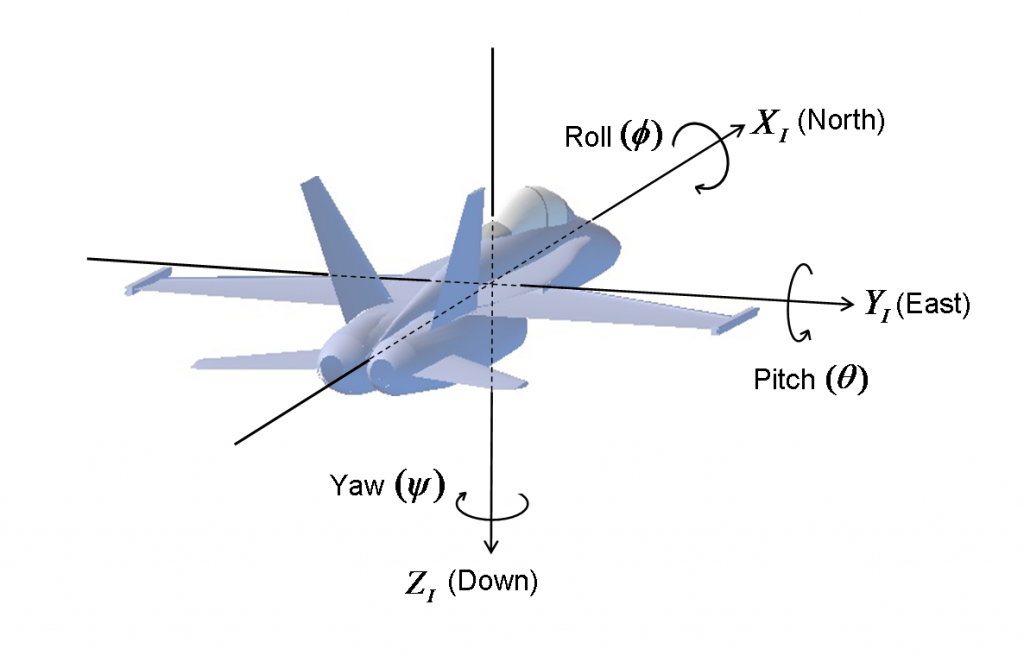
\includegraphics[width=0.6\linewidth]{image_euler_angles} \caption{Euler Angles}\label{fig:euler angles image}
\end{figure}

To convert quaternions to euler angles I used \emph{Q2EA} function from
\emph{orientlib} package.(See:
\url{https://www.rdocumentation.org/packages/orientlib/versions/0.10.3})

\begin{Shaded}
\begin{Highlighting}[]
\CommentTok{# define a function to convert quaternion values to euler angles. }
\NormalTok{convert_quaternions_to_euler <-}\StringTok{ }\ControlFlowTok{function}\NormalTok{(a_dataset)\{}
    
    \CommentTok{# use Q2EA from RSpincalc to convert quaternions to euler angles}
\NormalTok{    Q <-}\StringTok{ }\NormalTok{a_dataset }\OperatorTok\StringTok{ }\KeywordTok{select}\NormalTok{(}
\NormalTok{                    orientation_X, }
\NormalTok{                    orientation_Y, }
\NormalTok{                    orientation_Z, }
\NormalTok{                    orientation_W) }\OperatorTok\StringTok{ }
\StringTok{                }\KeywordTok{as.matrix}\NormalTok{()}
    
\NormalTok{    euler_matrix <-}\StringTok{ }\KeywordTok{Q2EA}\NormalTok{(Q, }
                 \DataTypeTok{EulerOrder=}\StringTok{'xyz'}\NormalTok{, }
                 \DataTypeTok{tol =} \DecValTok{10} \OperatorTok{*}\StringTok{ }\NormalTok{.Machine}\OperatorTok{$}\NormalTok{double.eps, }
                 \DataTypeTok{ichk =} \OtherTok{FALSE}\NormalTok{, }
                 \DataTypeTok{ignoreAllChk =} \OtherTok{FALSE}\NormalTok{)}

    \CommentTok{# add the new columns to the dataset}
\NormalTok{    a_dataset <-}\StringTok{ }\NormalTok{a_dataset }\OperatorTok\StringTok{ }\KeywordTok{mutate}\NormalTok{(}
                    \DataTypeTok{phi =}\NormalTok{ euler_matrix[,}\DecValTok{1}\NormalTok{],}
                    \DataTypeTok{theta =}\NormalTok{ euler_matrix[,}\DecValTok{2}\NormalTok{], }
                    \DataTypeTok{psi =}\NormalTok{ euler_matrix[,}\DecValTok{3}\NormalTok{])}
    
    \CommentTok{# remove quaternion columns}
\NormalTok{    a_dataset <-}\StringTok{ }\NormalTok{a_dataset }\OperatorTok\StringTok{ }\KeywordTok{select}\NormalTok{(}
                \OperatorTok{-}\NormalTok{orientation_X, }
                \OperatorTok{-}\NormalTok{orientation_Y,  }
                \OperatorTok{-}\NormalTok{orientation_Z, }
                \OperatorTok{-}\NormalTok{orientation_W)}
    
    \CommentTok{# return the new dataset}
\NormalTok{    a_dataset}
\NormalTok{\}}

\NormalTok{x_train <-}\StringTok{ }\KeywordTok{convert_quaternions_to_euler}\NormalTok{(x_train)}
\NormalTok{x_test <-}\StringTok{ }\KeywordTok{convert_quaternions_to_euler}\NormalTok{(x_test)}
\end{Highlighting}
\end{Shaded}

Distribution of orientation angles by surface:

\includegraphics{PH125_9_CYO_Report_files/figure-latex/euler distrib-1.pdf}

It looks like the most noticeable differences between surfaces can be
observed in the orientation distribution.

If we consider unit of time to be 1, we can draw the path of the robot
movement. In the following figures I draw the path for several cases,
faceted by surface. I expect that the surface would influence the shape
of these paths.

\includegraphics{PH125_9_CYO_Report_files/figure-latex/draw path-1.pdf}
\includegraphics{PH125_9_CYO_Report_files/figure-latex/draw path-2.pdf}

I cannot observe obvious differences between paths on carpet vs
concrete, but maybe a machine can. An idea would be to convert all paths
to images and do an image analysis, but I will stick with a more
classical approach for this project. I'll use several models from caret
package: \emph{KNN}, \emph{rpart} and \emph{randomForest.}

\hypertarget{data-pre-processing}{%
\subsection{Data Pre-Processing}\label{data-pre-processing}}

An important step in fitting a good model is pre-processing the data. In
our case we have series of observation of 128 measurements. In this
section I will create aggregations around these measurements. These are:
mean, standard deviation, distances of segments from one point to the
next. total distance, total angle change both from magnetostatic and
gyro sensors. All of these are encapsulated in the following function:

\begin{Shaded}
\begin{Highlighting}[]
\CommentTok{# function for pre-processing }
\CommentTok{# n_of_rows defaults to total number ofseries}
\CommentTok{# is_train indicates that the data is training, thus will do an extra action}
\NormalTok{pre_process <-}\StringTok{ }\ControlFlowTok{function}\NormalTok{(a_dataframe, }\DataTypeTok{n_of_rows =} \KeywordTok{nrow}\NormalTok{(a_dataframe)}\OperatorTok{/}\DecValTok{128}\NormalTok{ ) \{}
    
    \CommentTok{# get data grouped by seeries_id and compute some means }
\NormalTok{    processed_data_df <-}\StringTok{ }\NormalTok{a_dataframe }\OperatorTok\StringTok{ }
\StringTok{    }\KeywordTok{group_by}\NormalTok{(series_id) }\OperatorTok\StringTok{ }
\StringTok{    }\KeywordTok{summarize}\NormalTok{(}
        \DataTypeTok{phi_mean_all =} \KeywordTok{mean}\NormalTok{(phi),}
        \DataTypeTok{phi_sd_all =} \KeywordTok{sd}\NormalTok{(phi),}
        \DataTypeTok{phi_mean_to_sd_all =} \KeywordTok{mean}\NormalTok{(phi)}\OperatorTok{/}\KeywordTok{sd}\NormalTok{(phi),}
        \DataTypeTok{theta_mean_all =} \KeywordTok{mean}\NormalTok{(theta),}
        \DataTypeTok{theta_sd_all =} \KeywordTok{sd}\NormalTok{(theta),}
        \DataTypeTok{theta_mean_to_sd_all =} \KeywordTok{mean}\NormalTok{(theta)}\OperatorTok{/}\KeywordTok{sd}\NormalTok{(theta),}
        \DataTypeTok{psi_mean_all =} \KeywordTok{mean}\NormalTok{(psi),}
        \DataTypeTok{psi_sd_all =} \KeywordTok{sd}\NormalTok{(psi),}
        \DataTypeTok{psi_mean_to_sd_all =} \KeywordTok{mean}\NormalTok{(psi)}\OperatorTok{/}\KeywordTok{sd}\NormalTok{(psi),}
        \CommentTok{# this is the rectangular area that surounds the path of linear movement}
        \DataTypeTok{dist_area =}\NormalTok{ (}\KeywordTok{max}\NormalTok{(linear_acceleration_X) }\OperatorTok{-}\StringTok{ }\KeywordTok{min}\NormalTok{(linear_acceleration_X)) }\OperatorTok{*}\StringTok{ }\NormalTok{(}\KeywordTok{max}\NormalTok{(linear_acceleration_Y) }\OperatorTok{-}\StringTok{ }\KeywordTok{min}\NormalTok{(linear_acceleration_Y)) }\OperatorTok{+}\StringTok{ }
\StringTok{            }\NormalTok{(}\KeywordTok{max}\NormalTok{(linear_acceleration_X) }\OperatorTok{-}\StringTok{ }\KeywordTok{min}\NormalTok{(linear_acceleration_X)) }\OperatorTok{*}\StringTok{ }\NormalTok{(}\KeywordTok{max}\NormalTok{(linear_acceleration_Z) }\OperatorTok{-}\StringTok{ }\KeywordTok{min}\NormalTok{(linear_acceleration_Z)) }\OperatorTok{+}\StringTok{ }
\StringTok{            }\NormalTok{(}\KeywordTok{max}\NormalTok{(linear_acceleration_Y) }\OperatorTok{-}\StringTok{ }\KeywordTok{min}\NormalTok{(linear_acceleration_Y)) }\OperatorTok{*}\StringTok{ }\NormalTok{(}\KeywordTok{max}\NormalTok{(linear_acceleration_Z) }\OperatorTok{-}\StringTok{ }\KeywordTok{min}\NormalTok{(linear_acceleration_Z)),}
        \CommentTok{# this is the rectangular area that surounds the path of angular movement}
        \DataTypeTok{omega_area =}\NormalTok{ (}\KeywordTok{max}\NormalTok{(angular_velocity_X) }\OperatorTok{-}\StringTok{ }\KeywordTok{min}\NormalTok{(angular_velocity_X)) }\OperatorTok{*}\StringTok{ }\NormalTok{(}\KeywordTok{max}\NormalTok{(angular_velocity_Y) }\OperatorTok{-}\StringTok{ }\KeywordTok{min}\NormalTok{(angular_velocity_Y)) }\OperatorTok{+}
\StringTok{            }\NormalTok{(}\KeywordTok{max}\NormalTok{(angular_velocity_X) }\OperatorTok{-}\StringTok{ }\KeywordTok{min}\NormalTok{(angular_velocity_X)) }\OperatorTok{*}\StringTok{ }\NormalTok{(}\KeywordTok{max}\NormalTok{(angular_velocity_Z) }\OperatorTok{-}\StringTok{ }\KeywordTok{min}\NormalTok{(angular_velocity_Z)) }\OperatorTok{+}
\StringTok{            }\NormalTok{(}\KeywordTok{max}\NormalTok{(angular_velocity_Y) }\OperatorTok{-}\StringTok{ }\KeywordTok{min}\NormalTok{(angular_velocity_Y)) }\OperatorTok{*}\StringTok{ }\NormalTok{(}\KeywordTok{max}\NormalTok{(angular_velocity_Z) }\OperatorTok{-}\StringTok{ }\KeywordTok{min}\NormalTok{(angular_velocity_Z)),}
        \DataTypeTok{euler_area =}\NormalTok{ (}\KeywordTok{max}\NormalTok{(phi) }\OperatorTok{-}\StringTok{ }\KeywordTok{min}\NormalTok{(phi)) }\OperatorTok{*}\StringTok{ }\NormalTok{(}\KeywordTok{max}\NormalTok{(theta) }\OperatorTok{-}\StringTok{ }\KeywordTok{min}\NormalTok{(theta)) }\OperatorTok{+}\StringTok{ }
\StringTok{            }\NormalTok{(}\KeywordTok{max}\NormalTok{(phi) }\OperatorTok{-}\StringTok{ }\KeywordTok{min}\NormalTok{(phi)) }\OperatorTok{*}\StringTok{ }\NormalTok{(}\KeywordTok{max}\NormalTok{(psi) }\OperatorTok{-}\StringTok{ }\KeywordTok{min}\NormalTok{(psi)) }\OperatorTok{+}\StringTok{ }
\StringTok{            }\NormalTok{(}\KeywordTok{max}\NormalTok{(theta) }\OperatorTok{-}\StringTok{ }\KeywordTok{min}\NormalTok{(theta)) }\OperatorTok{*}\StringTok{ }\NormalTok{(}\KeywordTok{max}\NormalTok{(psi) }\OperatorTok{-}\StringTok{ }\KeywordTok{min}\NormalTok{(psi)),}
        \DataTypeTok{dist_mean_x =} \KeywordTok{mean}\NormalTok{(linear_acceleration_X),}
        \DataTypeTok{dist_mean_y =} \KeywordTok{mean}\NormalTok{(linear_acceleration_Y),}
        \DataTypeTok{dist_mean_z =} \KeywordTok{mean}\NormalTok{(linear_acceleration_Z),}
        \DataTypeTok{omega_mean_x =} \KeywordTok{mean}\NormalTok{(angular_velocity_X),}
        \DataTypeTok{omega_mean_y =} \KeywordTok{mean}\NormalTok{(angular_velocity_Y),}
        \DataTypeTok{omega_mean_Z =} \KeywordTok{mean}\NormalTok{(angular_velocity_Z),}
        \DataTypeTok{dist_sd_x =} \KeywordTok{sd}\NormalTok{(linear_acceleration_X),}
        \DataTypeTok{dist_sd_y =} \KeywordTok{sd}\NormalTok{(linear_acceleration_Y),}
        \DataTypeTok{dist_sd_z =} \KeywordTok{sd}\NormalTok{(linear_acceleration_Z),}
        \DataTypeTok{omega_sd_x =} \KeywordTok{sd}\NormalTok{(angular_velocity_X),}
        \DataTypeTok{omega_sd_y =} \KeywordTok{sd}\NormalTok{(angular_velocity_Y),}
        \DataTypeTok{omega_sd_Z =} \KeywordTok{sd}\NormalTok{(angular_velocity_Z) }
        
\NormalTok{        ) }\OperatorTok\StringTok{ }
\StringTok{        }\KeywordTok{slice}\NormalTok{(}\DecValTok{1}\OperatorTok{:}\NormalTok{n_of_rows)}
    
    \CommentTok{# define an empty data frame with summary metrics that we'll use for each set of 128 observations}
\NormalTok{    metrics <-}\StringTok{ }\KeywordTok{c}\NormalTok{(}\StringTok{"dist_total"}\NormalTok{,}\StringTok{"dist_max"}\NormalTok{,}\StringTok{"dist_min"}\NormalTok{,}\StringTok{"dist_max_to_min"}\NormalTok{,}\StringTok{"dist_mean"}\NormalTok{,}\StringTok{"dist_sd"}\NormalTok{,}\StringTok{"dist_mean_to_sd"}\NormalTok{,}
                             \StringTok{"omega_total"}\NormalTok{,}\StringTok{"omega_max"}\NormalTok{,}\StringTok{"omega_min"}\NormalTok{,}\StringTok{"omega_max_to_min"}\NormalTok{,}\StringTok{"omega_mean"}\NormalTok{,}\StringTok{"omega_sd"}\NormalTok{,}\StringTok{"omega_mean_to_sd"}\NormalTok{,}
                             \StringTok{"phi_total"}\NormalTok{,}\StringTok{"phi_max"}\NormalTok{,}\StringTok{"phi_min"}\NormalTok{,}\StringTok{"phi_mean"}\NormalTok{,}\StringTok{"phi_sd"}\NormalTok{,}\StringTok{"phi_mean_to_sd"}\NormalTok{,}
                             \StringTok{"theta_total"}\NormalTok{,}\StringTok{"theta_max"}\NormalTok{,}\StringTok{"theta_min"}\NormalTok{,}\StringTok{"theta_mean"}\NormalTok{,}\StringTok{"theta_sd"}\NormalTok{,}\StringTok{"theta_mean_to_sd"}\NormalTok{,}
                             \StringTok{"psi_total"}\NormalTok{,}\StringTok{"psi_max"}\NormalTok{,}\StringTok{"psi_min"}\NormalTok{,}\StringTok{"psi_mean"}\NormalTok{,}\StringTok{"psi_sd"}\NormalTok{,}\StringTok{"psi_mean_to_sd"}\NormalTok{,}
                             \StringTok{"euler_total"}\NormalTok{,}\StringTok{"euler_max"}\NormalTok{,}\StringTok{"euler_min"}\NormalTok{,}\StringTok{"euler_mean"}\NormalTok{,}\StringTok{"euler_sd"}\NormalTok{,}\StringTok{"euler_mean_to_sd"}\NormalTok{)}
\NormalTok{    tmp_df <-}\StringTok{ }\KeywordTok{data.frame}\NormalTok{(}\KeywordTok{matrix}\NormalTok{(}\DataTypeTok{ncol =} \KeywordTok{length}\NormalTok{(metrics), }\DataTypeTok{nrow =} \DecValTok{0}\NormalTok{) )}
    \KeywordTok{colnames}\NormalTok{(tmp_df) <-}\StringTok{ }\NormalTok{metrics}

    \CommentTok{# loop over each series and compute aggegations}
    \CommentTok{# should use apply type of function here, but I use "for" until I master the apply}
    \ControlFlowTok{for}\NormalTok{ (s_id }\ControlFlowTok{in}\NormalTok{ processed_data_df}\OperatorTok{$}\NormalTok{series_id)}
\NormalTok{    \{}
        \CommentTok{# get current measurement set}
\NormalTok{        this_chunk_df <-}\StringTok{ }\NormalTok{a_dataframe }\OperatorTok\StringTok{ }\KeywordTok{filter}\NormalTok{(series_id }\OperatorTok{==}\StringTok{ }\NormalTok{s_id)}
        
        \CommentTok{# select only columns we are interested in }
\NormalTok{        this_chunk_df <-}\StringTok{ }\NormalTok{this_chunk_df }\OperatorTok\StringTok{ }
\StringTok{            }\KeywordTok{select}\NormalTok{(}
\NormalTok{            phi, theta, psi,  }
\NormalTok{            angular_velocity_X, angular_velocity_Y, angular_velocity_Z,}
\NormalTok{            linear_acceleration_X, linear_acceleration_Y, linear_acceleration_Z)}
        \CommentTok{# this is a vector with euclidian distances from one point to the next}
\NormalTok{        dist_v <-}\StringTok{   }\KeywordTok{sqrt}\NormalTok{(}\KeywordTok{diff}\NormalTok{(this_chunk_df}\OperatorTok{$}\NormalTok{linear_acceleration_X)}\OperatorTok{^}\DecValTok{2} \OperatorTok{+}\StringTok{ }
\StringTok{                                }\KeywordTok{diff}\NormalTok{(this_chunk_df}\OperatorTok{$}\NormalTok{linear_acceleration_Y)}\OperatorTok{^}\DecValTok{2} \OperatorTok{+}\StringTok{ }
\StringTok{                                }\KeywordTok{diff}\NormalTok{(this_chunk_df}\OperatorTok{$}\NormalTok{linear_acceleration_Z)}\OperatorTok{^}\DecValTok{2}\NormalTok{)}
\NormalTok{        omega_v <-}\StringTok{  }\KeywordTok{sqrt}\NormalTok{(}\KeywordTok{diff}\NormalTok{(this_chunk_df}\OperatorTok{$}\NormalTok{angular_velocity_X)}\OperatorTok{^}\DecValTok{2} \OperatorTok{+}\StringTok{ }
\StringTok{                                }\KeywordTok{diff}\NormalTok{(this_chunk_df}\OperatorTok{$}\NormalTok{angular_velocity_Y)}\OperatorTok{^}\DecValTok{2} \OperatorTok{+}\StringTok{ }
\StringTok{                                }\KeywordTok{diff}\NormalTok{(this_chunk_df}\OperatorTok{$}\NormalTok{angular_velocity_Z)}\OperatorTok{^}\DecValTok{2}\NormalTok{)}
\NormalTok{        phi_v <-}\StringTok{ }\KeywordTok{abs}\NormalTok{(}\KeywordTok{diff}\NormalTok{(this_chunk_df}\OperatorTok{$}\NormalTok{phi))}
\NormalTok{        theta_v <-}\StringTok{ }\KeywordTok{abs}\NormalTok{(}\KeywordTok{diff}\NormalTok{(this_chunk_df}\OperatorTok{$}\NormalTok{theta))}
\NormalTok{        psi_v <-}\StringTok{ }\KeywordTok{abs}\NormalTok{(}\KeywordTok{diff}\NormalTok{(this_chunk_df}\OperatorTok{$}\NormalTok{psi))}

        \CommentTok{# fill or temp data frame with summary computations for our 128 measurement set}
\NormalTok{        tmp_df <-}\StringTok{ }\KeywordTok{bind_rows}\NormalTok{(tmp_df, }\KeywordTok{data_frame}\NormalTok{(}
            
            \CommentTok{# all features starting with "dist_" refers to linear movement}
            \DataTypeTok{dist_total =} \KeywordTok{sum}\NormalTok{(dist_v),}
            \DataTypeTok{dist_max =} \KeywordTok{max}\NormalTok{(dist_v),}
            \DataTypeTok{dist_min =} \KeywordTok{min}\NormalTok{(dist_v),}
            \DataTypeTok{dist_max_to_min =} \KeywordTok{max}\NormalTok{(dist_v)}\OperatorTok{/}\KeywordTok{min}\NormalTok{(dist_v),}
            \DataTypeTok{dist_mean =} \KeywordTok{mean}\NormalTok{(dist_v),}
            \DataTypeTok{dist_sd =} \KeywordTok{sd}\NormalTok{(dist_v),}
            \DataTypeTok{dist_mean_to_sd =} \KeywordTok{mean}\NormalTok{(dist_v)}\OperatorTok{/}\KeywordTok{sd}\NormalTok{(dist_v),  }\CommentTok{# reciprocal coef of variation}
            
            \CommentTok{# all features starting with "omega_" refers to angle velocity measurments}
            \DataTypeTok{omega_total =} \KeywordTok{sum}\NormalTok{(omega_v),}
            \DataTypeTok{omega_max =} \KeywordTok{max}\NormalTok{(omega_v),}
            \DataTypeTok{omega_min =} \KeywordTok{min}\NormalTok{(omega_v),}
            \DataTypeTok{omega_max_to_min =} \KeywordTok{max}\NormalTok{(omega_v)}\OperatorTok{/}\KeywordTok{min}\NormalTok{(omega_v),}
            \DataTypeTok{omega_mean =} \KeywordTok{mean}\NormalTok{(omega_v),}
            \DataTypeTok{omega_sd =} \KeywordTok{sd}\NormalTok{(omega_v),}
            \DataTypeTok{omega_mean_to_sd =} \KeywordTok{mean}\NormalTok{(omega_v)}\OperatorTok{/}\KeywordTok{sd}\NormalTok{(omega_v), }\CommentTok{# reciprocal coef of variation}

            \CommentTok{# phi, theta and psi reffers to roll, pitch and yaw rotations}
            \DataTypeTok{phi_total =} \KeywordTok{sum}\NormalTok{(phi_v),}
            \DataTypeTok{phi_max =} \KeywordTok{max}\NormalTok{(phi_v),}
            \DataTypeTok{phi_min =} \KeywordTok{min}\NormalTok{(phi_v),}
            \DataTypeTok{phi_mean =} \KeywordTok{mean}\NormalTok{(phi_v),}
            \DataTypeTok{phi_sd =} \KeywordTok{sd}\NormalTok{(phi_v),}
            \DataTypeTok{phi_mean_to_sd =} \KeywordTok{mean}\NormalTok{(phi_v)}\OperatorTok{/}\KeywordTok{sd}\NormalTok{(phi_v),}
            
            \DataTypeTok{theta_total =} \KeywordTok{sum}\NormalTok{(theta_v),}
            \DataTypeTok{theta_max =} \KeywordTok{max}\NormalTok{(theta_v),}
            \DataTypeTok{theta_min =} \KeywordTok{min}\NormalTok{(theta_v),}
            \DataTypeTok{theta_mean =} \KeywordTok{mean}\NormalTok{(theta_v),}
            \DataTypeTok{theta_sd =} \KeywordTok{sd}\NormalTok{(theta_v),}
            \DataTypeTok{theta_mean_to_sd =} \KeywordTok{mean}\NormalTok{(theta_v)}\OperatorTok{/}\KeywordTok{sd}\NormalTok{(theta_v),}
            
            \DataTypeTok{psi_total =} \KeywordTok{sum}\NormalTok{(psi_v),}
            \DataTypeTok{psi_max =} \KeywordTok{max}\NormalTok{(psi_v),}
            \DataTypeTok{psi_min =} \KeywordTok{min}\NormalTok{(psi_v),}
            \DataTypeTok{psi_mean =} \KeywordTok{mean}\NormalTok{(psi_v),}
            \DataTypeTok{psi_sd =} \KeywordTok{sd}\NormalTok{(psi_v),}
            \DataTypeTok{psi_mean_to_sd =} \KeywordTok{mean}\NormalTok{(psi_v)}\OperatorTok{/}\KeywordTok{sd}\NormalTok{(psi_v),}
            
            \CommentTok{# features starting with "euler_" refers to }
            \CommentTok{# agragation of all phi, theta and psi rotations}
            \DataTypeTok{euler_total =} \KeywordTok{sum}\NormalTok{(phi_v }\OperatorTok{+}\StringTok{ }\NormalTok{theta_v }\OperatorTok{+}\StringTok{ }\NormalTok{psi_v), }
            \DataTypeTok{euler_max =} \KeywordTok{max}\NormalTok{(phi_v }\OperatorTok{+}\StringTok{ }\NormalTok{theta_v }\OperatorTok{+}\StringTok{ }\NormalTok{psi_v),}
            \DataTypeTok{euler_min =} \KeywordTok{min}\NormalTok{(phi_v }\OperatorTok{+}\StringTok{ }\NormalTok{theta_v }\OperatorTok{+}\StringTok{ }\NormalTok{psi_v),}
            \DataTypeTok{euler_mean =} \KeywordTok{mean}\NormalTok{(phi_v }\OperatorTok{+}\StringTok{ }\NormalTok{theta_v }\OperatorTok{+}\StringTok{ }\NormalTok{psi_v),}
            \DataTypeTok{euler_sd =} \KeywordTok{sd}\NormalTok{(phi_v }\OperatorTok{+}\StringTok{ }\NormalTok{theta_v }\OperatorTok{+}\StringTok{ }\NormalTok{psi_v),}
            \DataTypeTok{euler_mean_to_sd =} \KeywordTok{mean}\NormalTok{(phi_v }\OperatorTok{+}\StringTok{ }\NormalTok{theta_v }\OperatorTok{+}\StringTok{ }\NormalTok{psi_v)}\OperatorTok{/}\KeywordTok{sd}\NormalTok{(phi_v }\OperatorTok{+}\StringTok{ }\NormalTok{theta_v }\OperatorTok{+}\StringTok{ }\NormalTok{psi_v)}
\NormalTok{            ))}
    
\NormalTok{    \} }\CommentTok{# end of for over series}
    
    \CommentTok{# add the summary computations to the data set of series}
\NormalTok{    processed_data_df <-}\StringTok{ }\KeywordTok{bind_cols}\NormalTok{(processed_data_df, tmp_df)}

    \CommentTok{# more features}
    \CommentTok{# I added thesee as an experimentation after observing the dependencies graphs}
    \CommentTok{# will explain later}
\NormalTok{    processed_data_df <-}\StringTok{ }\NormalTok{processed_data_df }\OperatorTok\StringTok{ }\KeywordTok{mutate}\NormalTok{(}
        \CommentTok{# this is an agular momentum }
        \DataTypeTok{f1 =} \KeywordTok{log}\NormalTok{(dist_mean_to_sd}\OperatorTok{*}\NormalTok{omega_mean_to_sd),}
        
        \CommentTok{# this is an angular momentum }
        \DataTypeTok{f2 =} \KeywordTok{log}\NormalTok{(dist_total}\OperatorTok{*}\NormalTok{omega_total),}
        
        \CommentTok{# this is the angle between theta and psi vectors}
        \DataTypeTok{f3 =} \KeywordTok{abs}\NormalTok{(}\KeywordTok{atan}\NormalTok{(theta_mean_all}\OperatorTok{/}\NormalTok{psi_mean_all)))        }
    
    \CommentTok{# return the proceessed data}
\NormalTok{    processed_data_df}
\NormalTok{\}}
\end{Highlighting}
\end{Shaded}

Pre-process the data and save it to a local file. This is to save time
for further analysis by skipping the pre-processing procedure. I'm using
\emph{tic()} \emph{toc()} functions from \emph{tictoc} package to
display processing time.

\begin{Shaded}
\begin{Highlighting}[]
\CommentTok{# pre-process train and test data sets}
\KeywordTok{tic}\NormalTok{(}\StringTok{"process train data"}\NormalTok{)}
\NormalTok{x_train_processed <-}\StringTok{ }\KeywordTok{pre_process}\NormalTok{(x_train)}
\KeywordTok{toc}\NormalTok{()}
\end{Highlighting}
\end{Shaded}

\begin{verbatim}
## process train data: 46.08 sec elapsed
\end{verbatim}

\begin{Shaded}
\begin{Highlighting}[]
\KeywordTok{tic}\NormalTok{(}\StringTok{"process test data"}\NormalTok{)}
\NormalTok{x_test_processed <-}\StringTok{ }\KeywordTok{pre_process}\NormalTok{(x_test)}
\KeywordTok{toc}\NormalTok{()}
\end{Highlighting}
\end{Shaded}

\begin{verbatim}
## process test data: 44.36 sec elapsed
\end{verbatim}

\begin{Shaded}
\begin{Highlighting}[]
\CommentTok{# rejoin train data with the labels data set}
\NormalTok{x_train_processed <-}\StringTok{ }\NormalTok{x_train_processed }\OperatorTok\StringTok{ }\KeywordTok{left_join}\NormalTok{(y_train, }\DataTypeTok{by =} \StringTok{"series_id"}\NormalTok{)}

\CommentTok{# create a folder "data" if doesnt exist}
\ControlFlowTok{if}\NormalTok{ (}\OperatorTok{!}\KeywordTok{dir.exists}\NormalTok{(}\StringTok{"data"}\NormalTok{)) }\KeywordTok{dir.create}\NormalTok{(}\StringTok{"data"}\NormalTok{)}

\CommentTok{# save processed data, and use these files from now on}
\KeywordTok{write_csv}\NormalTok{(x_train_processed, }\StringTok{"data/x_train_processed.csv"}\NormalTok{)}
\KeywordTok{write_csv}\NormalTok{(x_test_processed, }\StringTok{"data/x_test_processed.csv"}\NormalTok{)}

\CommentTok{# clean some variables and the environment}
\KeywordTok{rm}\NormalTok{(x_train, x_test, y_train)}
\KeywordTok{rm}\NormalTok{(x_train_processed, x_test_processed)}
\end{Highlighting}
\end{Shaded}

Load pre-processed data from hard-disk and use them from here. In this
report I will use a smaller data set from the training data, to make
things work faster. Full data set will be used in the final script

\begin{Shaded}
\begin{Highlighting}[]
\NormalTok{x_train_processed_from_file <-}\StringTok{ }\KeywordTok{read_csv}\NormalTok{(}\StringTok{"data/x_train_processed.csv"}\NormalTok{)}
\NormalTok{x_test_processed_from_file <-}\StringTok{ }\KeywordTok{read_csv}\NormalTok{(}\StringTok{"data/x_test_processed.csv"}\NormalTok{)}

\CommentTok{# if we load data from a file, convert surface to factor}
\NormalTok{x_train_processed_from_file <-}\StringTok{ }\NormalTok{x_train_processed_from_file }\OperatorTok\StringTok{ }\KeywordTok{mutate}\NormalTok{(}\DataTypeTok{surface =} \KeywordTok{as.factor}\NormalTok{(surface))}

\CommentTok{# use a smaller set of datab to save time}
\NormalTok{x_train_processed_from_file <-}\StringTok{ }\NormalTok{x_train_processed_from_file }\OperatorTok\StringTok{  }\KeywordTok{slice}\NormalTok{(}\DecValTok{1}\OperatorTok{:}\DecValTok{1200}\NormalTok{)}
\end{Highlighting}
\end{Shaded}

\hypertarget{correlated-predictors}{%
\subsection{Correlated Predictors}\label{correlated-predictors}}

\begin{Shaded}
\begin{Highlighting}[]
\CommentTok{# from now we can load pre-processed data from csv files without the need to pre-process again}
\NormalTok{x_test_processed <-}\StringTok{ }\NormalTok{x_test_processed_from_file}
\NormalTok{x_train_processed <-}\StringTok{ }\NormalTok{x_train_processed_from_file }
\end{Highlighting}
\end{Shaded}

We created 65 features, lets trim some of them. First, I will identify
those that are strongly correlated. Lets plot the correlation matrix:

\begin{Shaded}
\begin{Highlighting}[]
\KeywordTok{library}\NormalTok{(RColorBrewer)}
\KeywordTok{library}\NormalTok{(corrplot)}
\NormalTok{x_matrix <-}\StringTok{ }\NormalTok{x_train_processed }\OperatorTok\StringTok{ }\KeywordTok{select}\NormalTok{(}\OperatorTok{-}\NormalTok{series_id, }\OperatorTok{-}\NormalTok{group_id, }\OperatorTok{-}\NormalTok{surface) }\OperatorTok\StringTok{ }
\StringTok{    }\KeywordTok{as.matrix}\NormalTok{()}
\NormalTok{x_cor <-}\StringTok{ }\KeywordTok{cor}\NormalTok{(x_matrix, }\DataTypeTok{use =} \StringTok{"pairwise.complete"}\NormalTok{)}
\KeywordTok{corrplot}\NormalTok{(x_cor,}\DataTypeTok{method =} \StringTok{"square"}\NormalTok{, }\DataTypeTok{number.cex =} \FloatTok{.5}\NormalTok{, }\DataTypeTok{tl.cex =} \FloatTok{0.6}\NormalTok{ ,}\DataTypeTok{order =} \StringTok{"hclust"}\NormalTok{,  }\DataTypeTok{title =} \StringTok{"Correlation Matrix"}\NormalTok{)}
\end{Highlighting}
\end{Shaded}

\includegraphics{PH125_9_CYO_Report_files/figure-latex/correlation matrix before-1.pdf}

\begin{Shaded}
\begin{Highlighting}[]
\KeywordTok{rm}\NormalTok{(x_matrix, x_cor)}
\end{Highlighting}
\end{Shaded}

Using function \emph{findCorrelation} from \emph{caret} we can remove
features that are highly correlated

\begin{Shaded}
\begin{Highlighting}[]
\CommentTok{# convert both test and train data to matrix in order to analyse feature corelation}
\NormalTok{x_train_matrix <-}\StringTok{ }\NormalTok{x_train_processed }\OperatorTok\StringTok{ }\KeywordTok{select}\NormalTok{(}\OperatorTok{-}\NormalTok{surface, }\OperatorTok{-}\NormalTok{series_id) }\OperatorTok\StringTok{ }\KeywordTok{as.matrix}\NormalTok{()}
\NormalTok{x_test_matrix <-}\StringTok{ }\NormalTok{x_test_processed }\OperatorTok\StringTok{ }\KeywordTok{select}\NormalTok{(}\OperatorTok{-}\NormalTok{series_id) }\OperatorTok\StringTok{ }\KeywordTok{as.matrix}\NormalTok{()}

\CommentTok{# find features that are high correlated }
\CommentTok{# find linear dependencies and eliminate them}
\NormalTok{names_to_remove_test <-}\StringTok{ }\KeywordTok{findCorrelation}\NormalTok{(}\KeywordTok{cor}\NormalTok{(x_test_matrix), }\DataTypeTok{cutoff =} \FloatTok{0.95}\NormalTok{, }\DataTypeTok{names =} \OtherTok{TRUE}\NormalTok{, }\DataTypeTok{verbose =} \OtherTok{FALSE}\NormalTok{, }\DataTypeTok{exact=}\OtherTok{TRUE}\NormalTok{)}

\CommentTok{# remove correlated features from both train and test sets}
\NormalTok{x_train_processed <-}\StringTok{ }\NormalTok{x_train_processed }\OperatorTok\StringTok{ }\KeywordTok{select}\NormalTok{(}\OperatorTok{-}\NormalTok{names_to_remove_test) }
\NormalTok{x_test_processed <-}\StringTok{ }\NormalTok{x_test_processed }\OperatorTok\StringTok{ }\KeywordTok{select}\NormalTok{(}\OperatorTok{-}\NormalTok{names_to_remove_test) }

\CommentTok{# draw again the correlation matrix}
\NormalTok{x_matrix <-}\StringTok{ }\NormalTok{x_train_processed }\OperatorTok\StringTok{ }\KeywordTok{select}\NormalTok{(}\OperatorTok{-}\NormalTok{series_id, }\OperatorTok{-}\NormalTok{group_id, }\OperatorTok{-}\NormalTok{surface) }\OperatorTok\StringTok{ }
\StringTok{    }\KeywordTok{as.matrix}\NormalTok{()}
\NormalTok{x_cor <-}\StringTok{ }\KeywordTok{cor}\NormalTok{(x_matrix, }\DataTypeTok{use =} \StringTok{"pairwise.complete"}\NormalTok{)}
\KeywordTok{corrplot}\NormalTok{(x_cor,}\DataTypeTok{method =} \StringTok{"square"}\NormalTok{, }\DataTypeTok{number.cex =} \FloatTok{.5}\NormalTok{, }\DataTypeTok{tl.cex =} \FloatTok{0.6}\NormalTok{ ,}\DataTypeTok{order =} \StringTok{"hclust"}\NormalTok{,  }\DataTypeTok{title =} \StringTok{"Correlation Matrix"}\NormalTok{)}
\end{Highlighting}
\end{Shaded}

\includegraphics{PH125_9_CYO_Report_files/figure-latex/correlation matrix after-1.pdf}

\begin{Shaded}
\begin{Highlighting}[]
\KeywordTok{rm}\NormalTok{(x_train_matrix, x_test_matrix, x_matrix, x_cor)}
\end{Highlighting}
\end{Shaded}

The number of predictors decreased to 42

Another useful technique in pre-processing is centering around means and
scaling the predictors:

\begin{Shaded}
\begin{Highlighting}[]
\CommentTok{# pre-process the data, center and scale the values across all predictors}
\NormalTok{pre_process <-}\StringTok{ }\NormalTok{x_train_processed }\OperatorTok\StringTok{ }\KeywordTok{select}\NormalTok{(}\OperatorTok{-}\NormalTok{series_id, }\OperatorTok{-}\NormalTok{group_id) }\OperatorTok\StringTok{ }\KeywordTok{preProcess}\NormalTok{(}\DataTypeTok{method =} \KeywordTok{c}\NormalTok{(}\StringTok{"center"}\NormalTok{, }\StringTok{"scale"}\NormalTok{))}
\NormalTok{x_train_processed <-}\StringTok{ }\KeywordTok{predict}\NormalTok{(pre_process, x_train_processed)}
\NormalTok{x_test_processed <-}\StringTok{ }\KeywordTok{predict}\NormalTok{(pre_process, x_test_processed)}

\KeywordTok{rm}\NormalTok{(pre_process)}
\end{Highlighting}
\end{Shaded}

\hypertarget{data-visualization}{%
\subsection{Data Visualization}\label{data-visualization}}

Before moving forward with more feature selection, I will plot some
interesting visualizations of the feature dependencies. These are plots
of orientation angles as sums over all 128 points. \emph{phi},
\emph{theta} and \emph{psi} are euler orientation angles.

\begin{Shaded}
\begin{Highlighting}[]
\NormalTok{x_train_processed }\OperatorTok\StringTok{  }\KeywordTok{ggplot}\NormalTok{(}\KeywordTok{aes}\NormalTok{(phi_mean_all, psi_mean_all, }\DataTypeTok{fill =}\NormalTok{ surface)) }\OperatorTok{+}
\StringTok{    }\KeywordTok{geom_point}\NormalTok{(}\KeywordTok{aes}\NormalTok{(}\DataTypeTok{color =}\NormalTok{ surface)) }\OperatorTok{+}\StringTok{ }
\StringTok{    }\KeywordTok{geom_point}\NormalTok{(}\DataTypeTok{cex=}\DecValTok{6}\NormalTok{, }\DataTypeTok{pch=}\DecValTok{21}\NormalTok{) }\OperatorTok{+}
\StringTok{    }\KeywordTok{ggtitle}\NormalTok{(}\StringTok{"phi_mean vs. psi_mean"}\NormalTok{)}
\end{Highlighting}
\end{Shaded}

\includegraphics{PH125_9_CYO_Report_files/figure-latex/euler visualizations-1.pdf}

\begin{Shaded}
\begin{Highlighting}[]
\NormalTok{x_train_processed }\OperatorTok\StringTok{  }\KeywordTok{ggplot}\NormalTok{(}\KeywordTok{aes}\NormalTok{(theta_mean_all, psi_mean_all, }\DataTypeTok{fill =}\NormalTok{ surface)) }\OperatorTok{+}
\StringTok{    }\KeywordTok{geom_point}\NormalTok{(}\KeywordTok{aes}\NormalTok{(}\DataTypeTok{color =}\NormalTok{ surface)) }\OperatorTok{+}
\StringTok{    }\KeywordTok{geom_point}\NormalTok{(}\DataTypeTok{cex=}\DecValTok{6}\NormalTok{, }\DataTypeTok{pch=}\DecValTok{21}\NormalTok{) }\OperatorTok{+}\StringTok{ }
\StringTok{    }\KeywordTok{ggtitle}\NormalTok{(}\StringTok{"theta_mean vs. psi_mean"}\NormalTok{)}
\end{Highlighting}
\end{Shaded}

\includegraphics{PH125_9_CYO_Report_files/figure-latex/euler visualizations-2.pdf}

\begin{Shaded}
\begin{Highlighting}[]
\NormalTok{x_train_processed }\OperatorTok\StringTok{  }\KeywordTok{ggplot}\NormalTok{(}\KeywordTok{aes}\NormalTok{(theta_mean_all, phi_mean_all, }\DataTypeTok{fill =}\NormalTok{ surface)) }\OperatorTok{+}
\StringTok{    }\KeywordTok{geom_point}\NormalTok{(}\KeywordTok{aes}\NormalTok{(}\DataTypeTok{color =}\NormalTok{ surface)) }\OperatorTok{+}
\StringTok{    }\KeywordTok{geom_point}\NormalTok{(}\DataTypeTok{cex=}\DecValTok{6}\NormalTok{, }\DataTypeTok{pch=}\DecValTok{21}\NormalTok{) }\OperatorTok{+}
\StringTok{    }\KeywordTok{ggtitle}\NormalTok{(}\StringTok{"theta_mean vs. phi_mean"}\NormalTok{)}
\end{Highlighting}
\end{Shaded}

\includegraphics{PH125_9_CYO_Report_files/figure-latex/euler visualizations-3.pdf}
I would speculate that all points that are not on the global pattern are
actually outlines, but I did not explore that hypothesis.

The following is the angle between \emph{theta} - \emph{psi} vectors and
the angular momentum:

\begin{Shaded}
\begin{Highlighting}[]
\NormalTok{x_train_processed }\OperatorTok\StringTok{  }\KeywordTok{ggplot}\NormalTok{(}\KeywordTok{aes}\NormalTok{(f2, f3, }\DataTypeTok{fill =}\NormalTok{ surface)) }\OperatorTok{+}
\StringTok{    }\KeywordTok{geom_point}\NormalTok{(}\KeywordTok{aes}\NormalTok{(}\DataTypeTok{color =}\NormalTok{ surface)) }\OperatorTok{+}
\StringTok{    }\KeywordTok{geom_point}\NormalTok{(}\DataTypeTok{cex=}\DecValTok{6}\NormalTok{, }\DataTypeTok{pch=}\DecValTok{21}\NormalTok{) }\OperatorTok{+}
\StringTok{    }\KeywordTok{ggtitle}\NormalTok{(}\StringTok{"theta-psi angle vs. angular momentum"}\NormalTok{)}
\end{Highlighting}
\end{Shaded}

\includegraphics{PH125_9_CYO_Report_files/figure-latex/theta psi and momentum-1.pdf}
We can see some separations by surfaces that may allow a KNN model to
work. In fact if we run KNN for just \emph{surface \textasciitilde{} f2
+ f3} we will get an accuracy of 0.56 which is promising.

\hypertarget{more-feature-selection}{%
\subsection{More Feature Selection}\label{more-feature-selection}}

I will continue now removing more features based on their importance in
a randomForest model. I will split the training set into two partitions:
\emph{x\_train\_for\_train} used for training, and
\emph{x\_train\_for\_test} to measure the accuracy. Then will plot
variable importance. Will not use here any tuning, since this is not the
final model.

\begin{Shaded}
\begin{Highlighting}[]
\CommentTok{# partition x_train_processed data for training and testing }
\NormalTok{test_index <-}\StringTok{ }\KeywordTok{createDataPartition}\NormalTok{(}\DataTypeTok{y =}\NormalTok{ x_train_processed}\OperatorTok{$}\NormalTok{surface, }\DataTypeTok{times =} \DecValTok{1}\NormalTok{, }\DataTypeTok{p =} \FloatTok{0.5}\NormalTok{, }\DataTypeTok{list =} \OtherTok{FALSE}\NormalTok{)}
\NormalTok{x_train_for_train <-}\StringTok{ }\NormalTok{x_train_processed[}\OperatorTok{-}\NormalTok{test_index, ]}
\NormalTok{x_train_for_test <-}\StringTok{ }\NormalTok{x_train_processed[test_index, ]}
\KeywordTok{rm}\NormalTok{(test_index)}

\NormalTok{model_fit <-}\StringTok{ }\KeywordTok{randomForest}\NormalTok{(}
\NormalTok{    surface }\OperatorTok{~}\StringTok{ }\NormalTok{., }
    \DataTypeTok{metric =} \StringTok{"Accuracy"}\NormalTok{, }
    \CommentTok{# remove series_id, group_id and select only 500 points}
    \DataTypeTok{data =} \KeywordTok{slice}\NormalTok{(}\KeywordTok{select}\NormalTok{(x_train_for_train, }\OperatorTok{-}\NormalTok{series_id, }\OperatorTok{-}\NormalTok{group_id), }\DecValTok{1}\OperatorTok{:}\DecValTok{500}\NormalTok{)}
\NormalTok{    )}

\NormalTok{y_hat <-}\StringTok{ }\KeywordTok{predict}\NormalTok{(model_fit, }\KeywordTok{select}\NormalTok{(x_train_for_test, }\OperatorTok{-}\NormalTok{series_id))}
\NormalTok{y_test <-}\StringTok{ }\NormalTok{x_train_for_test}\OperatorTok{$}\NormalTok{surface}

\CommentTok{# # we dont show accuracy and confusion table for now}
\CommentTok{# conf_matrix <- confusionMatrix(y_hat, x_train_for_test$surface)}
\CommentTok{# conf_matrix$overall["Accuracy"]}
\CommentTok{# conf_matrix$table %>% knitr::kable()}

\NormalTok{importance <-}\StringTok{ }\KeywordTok{importance}\NormalTok{(model_fit)}
\NormalTok{importance <-}\StringTok{ }\NormalTok{importance[}\KeywordTok{order}\NormalTok{(importance[,}\DecValTok{1}\NormalTok{], }\DataTypeTok{decreasing =} \OtherTok{TRUE}\NormalTok{), ]}

\CommentTok{# plot variable importance}
\KeywordTok{varImpPlot}\NormalTok{(model_fit)}
\end{Highlighting}
\end{Shaded}

\includegraphics{PH125_9_CYO_Report_files/figure-latex/randomForest-1.pdf}

\begin{Shaded}
\begin{Highlighting}[]
\CommentTok{# this is the list of variables in order of importance, decreasing}
\NormalTok{features <-}\StringTok{ }\KeywordTok{names}\NormalTok{(importance)}
\end{Highlighting}
\end{Shaded}

We observe following variables does not help prediction too much:
\emph{theta\_min}, \emph{omega\_max\_to\_min}, \emph{dist\_mean\_y},
\emph{omega\_mean\_x}, \emph{dist\_mean\_x}, \emph{dist\_mean\_z} So I
will remove them:

\begin{Shaded}
\begin{Highlighting}[]
\CommentTok{# remove columns do not contribute to classification}
\NormalTok{x_train_processed <-}\StringTok{ }\NormalTok{x_train_processed }\OperatorTok\StringTok{ }\KeywordTok{select}\NormalTok{(}\OperatorTok{-}\NormalTok{theta_min, }\OperatorTok{-}\NormalTok{omega_max_to_min, }\OperatorTok{-}\NormalTok{dist_mean_y, }\OperatorTok{-}\NormalTok{omega_mean_x, }\OperatorTok{-}\NormalTok{dist_mean_x, }\OperatorTok{-}\NormalTok{dist_mean_z)}
\NormalTok{x_test_processed <-}\StringTok{ }\NormalTok{x_test_processed }\OperatorTok\StringTok{ }\KeywordTok{select}\NormalTok{(}\OperatorTok{-}\NormalTok{theta_min, }\OperatorTok{-}\NormalTok{omega_max_to_min, }\OperatorTok{-}\NormalTok{dist_mean_y, }\OperatorTok{-}\NormalTok{omega_mean_x, }\OperatorTok{-}\NormalTok{dist_mean_x, }\OperatorTok{-}\NormalTok{dist_mean_z)}
\end{Highlighting}
\end{Shaded}

\hypertarget{the-model}{%
\section{The Model}\label{the-model}}

It is time now to fit some models. I tried many models on the side but I
will present in this report only

\begin{itemize}
\tightlist
\item
  KNN,
\item
  rpart,
\item
  randomForest,
\item
  randomForest assembly
\end{itemize}

Please note that the code in this report is using only 1000 records from
training, that is further partitioned in train and test with 0.5 ratio
I've done this to make it run faster. I am using full data set in the R
script and also I will present the final results from Kaggle (i think I
said this before).

\hypertarget{knn-model}{%
\subsection{KNN Model}\label{knn-model}}

KNN is getting incrementally slower with the number of features. So for
KNN I used only the most important variables as part of the formula.

\begin{Shaded}
\begin{Highlighting}[]
\CommentTok{# use most important variables to fit KNN}
\NormalTok{model_fit <-}\StringTok{ }\KeywordTok{train}\NormalTok{(surface }\OperatorTok{~}\StringTok{ }\NormalTok{f3 }\OperatorTok{+}\StringTok{ }\NormalTok{f2 }\OperatorTok{+}\StringTok{ }\NormalTok{phi_mean_all }\OperatorTok{+}\StringTok{ }\NormalTok{theta_mean_all }\OperatorTok{+}\StringTok{ }\NormalTok{psi_mean_all,  }\DataTypeTok{method =} \StringTok{"knn"}\NormalTok{, }
             \DataTypeTok{tuneGrid =} \KeywordTok{data.frame}\NormalTok{(}\DataTypeTok{k =} \KeywordTok{seq}\NormalTok{(}\DecValTok{2}\NormalTok{, }\DecValTok{100}\NormalTok{, }\DecValTok{2}\NormalTok{)), }
             \DataTypeTok{data =} \KeywordTok{select}\NormalTok{(x_train_for_train, }\OperatorTok{-}\NormalTok{series_id, }\OperatorTok{-}\NormalTok{group_id))}

\KeywordTok{ggplot}\NormalTok{(model_fit) }
\end{Highlighting}
\end{Shaded}

\includegraphics{PH125_9_CYO_Report_files/figure-latex/KNN-1.pdf}

\begin{Shaded}
\begin{Highlighting}[]
\CommentTok{# get confusion matrix and display it together with the results}
\NormalTok{y_hat <-}\StringTok{ }\KeywordTok{predict}\NormalTok{(model_fit, }\KeywordTok{select}\NormalTok{(x_train_for_test, }\OperatorTok{-}\NormalTok{series_id, }\OperatorTok{-}\NormalTok{group_id), }\DataTypeTok{type =} \StringTok{"raw"}\NormalTok{)}
\NormalTok{conf_matrix <-}\StringTok{ }\KeywordTok{confusionMatrix}\NormalTok{(y_hat, x_train_for_test}\OperatorTok{$}\NormalTok{surface)}

\CommentTok{# display confusion matrix}
\NormalTok{conf_matrix}\OperatorTok{$}\NormalTok{table }\OperatorTok\StringTok{ }\NormalTok{knitr}\OperatorTok{::}\KeywordTok{kable}\NormalTok{()}
\end{Highlighting}
\end{Shaded}

\begin{longtable}[]{@{}lrrrrrrrrr@{}}
\toprule
& carpet & concrete & fine\_concrete & hard\_tiles &
hard\_tiles\_large\_space & soft\_pvc & soft\_tiles & tiled &
wood\tabularnewline
\midrule
\endhead
carpet & 20 & 4 & 0 & 0 & 0 & 5 & 0 & 2 & 2\tabularnewline
concrete & 5 & 84 & 0 & 0 & 0 & 5 & 0 & 6 & 5\tabularnewline
fine\_concrete & 0 & 0 & 33 & 0 & 5 & 1 & 1 & 2 & 3\tabularnewline
hard\_tiles & 1 & 0 & 0 & 7 & 0 & 0 & 0 & 0 & 0\tabularnewline
hard\_tiles\_large\_space & 0 & 2 & 0 & 0 & 23 & 2 & 0 & 1 &
3\tabularnewline
soft\_pvc & 4 & 4 & 4 & 0 & 2 & 114 & 7 & 5 & 3\tabularnewline
soft\_tiles & 1 & 1 & 4 & 0 & 6 & 8 & 91 & 1 & 0\tabularnewline
tiled & 7 & 5 & 0 & 1 & 0 & 0 & 2 & 42 & 5\tabularnewline
wood & 0 & 2 & 2 & 0 & 1 & 2 & 1 & 9 & 47\tabularnewline
\bottomrule
\end{longtable}

\begin{Shaded}
\begin{Highlighting}[]
\CommentTok{# create a data frame to store Accuracy results by model}
\NormalTok{model_results <-}\StringTok{ }\KeywordTok{data.frame}\NormalTok{(}\DataTypeTok{Model =} \StringTok{"KNN"}\NormalTok{, }\DataTypeTok{Accuracy =}\NormalTok{ conf_matrix}\OperatorTok{$}\NormalTok{overall[}\StringTok{"Accuracy"}\NormalTok{])}
\NormalTok{model_results }\OperatorTok\StringTok{ }\NormalTok{knitr}\OperatorTok{::}\KeywordTok{kable}\NormalTok{()}
\end{Highlighting}
\end{Shaded}

\begin{longtable}[]{@{}llr@{}}
\toprule
& Model & Accuracy\tabularnewline
\midrule
\endhead
Accuracy & KNN & 0.7645108\tabularnewline
\bottomrule
\end{longtable}

\hypertarget{rpart-model}{%
\subsection{rpart Model}\label{rpart-model}}

Another model I tried is rpart (Recursive Partitioning And Regression
Tree). I will tune it on the complexity coeficient

\begin{Shaded}
\begin{Highlighting}[]
\NormalTok{model_fit <-}\StringTok{ }\KeywordTok{train}\NormalTok{(surface }\OperatorTok{~}\StringTok{ }\NormalTok{., }
                     \DataTypeTok{method =} \StringTok{"rpart"}\NormalTok{,}
                     \DataTypeTok{tuneGrid =} \KeywordTok{data.frame}\NormalTok{(}\DataTypeTok{cp =} \KeywordTok{seq}\NormalTok{(}\DecValTok{0}\NormalTok{, }\FloatTok{0.075}\NormalTok{, }\DataTypeTok{len =} \DecValTok{40}\NormalTok{)),}
                     \DataTypeTok{data =} \KeywordTok{select}\NormalTok{(x_train_for_train, }\OperatorTok{-}\NormalTok{series_id, }\OperatorTok{-}\NormalTok{group_id))}
\KeywordTok{ggplot}\NormalTok{(model_fit)}
\end{Highlighting}
\end{Shaded}

\includegraphics{PH125_9_CYO_Report_files/figure-latex/rpart-1.pdf}

\begin{Shaded}
\begin{Highlighting}[]
\CommentTok{# get confusion matrix and display it together with the results}
\NormalTok{y_hat <-}\StringTok{ }\KeywordTok{predict}\NormalTok{(model_fit, }\KeywordTok{select}\NormalTok{(x_train_for_test, }\OperatorTok{-}\NormalTok{series_id, }\OperatorTok{-}\NormalTok{group_id), }\DataTypeTok{type =} \StringTok{"raw"}\NormalTok{)}
\NormalTok{conf_matrix <-}\StringTok{ }\KeywordTok{confusionMatrix}\NormalTok{(y_hat, x_train_for_test}\OperatorTok{$}\NormalTok{surface)}

\CommentTok{# display confusion matrix}
\NormalTok{conf_matrix}\OperatorTok{$}\NormalTok{table }\OperatorTok\StringTok{ }\NormalTok{knitr}\OperatorTok{::}\KeywordTok{kable}\NormalTok{()}
\end{Highlighting}
\end{Shaded}

\begin{longtable}[]{@{}lrrrrrrrrr@{}}
\toprule
& carpet & concrete & fine\_concrete & hard\_tiles &
hard\_tiles\_large\_space & soft\_pvc & soft\_tiles & tiled &
wood\tabularnewline
\midrule
\endhead
carpet & 11 & 4 & 0 & 0 & 1 & 3 & 0 & 3 & 9\tabularnewline
concrete & 3 & 83 & 0 & 0 & 0 & 3 & 0 & 2 & 4\tabularnewline
fine\_concrete & 0 & 0 & 28 & 1 & 0 & 4 & 2 & 1 & 4\tabularnewline
hard\_tiles & 1 & 2 & 5 & 7 & 1 & 0 & 0 & 1 & 0\tabularnewline
hard\_tiles\_large\_space & 0 & 2 & 0 & 0 & 23 & 3 & 0 & 5 &
5\tabularnewline
soft\_pvc & 17 & 4 & 5 & 0 & 0 & 116 & 11 & 11 & 4\tabularnewline
soft\_tiles & 0 & 0 & 5 & 0 & 10 & 8 & 85 & 0 & 0\tabularnewline
tiled & 2 & 0 & 0 & 0 & 0 & 0 & 4 & 40 & 6\tabularnewline
wood & 4 & 7 & 0 & 0 & 2 & 0 & 0 & 5 & 36\tabularnewline
\bottomrule
\end{longtable}

\begin{Shaded}
\begin{Highlighting}[]
\NormalTok{model_results <-}\StringTok{ }\KeywordTok{bind_rows}\NormalTok{(model_results,}
                           \KeywordTok{data_frame}\NormalTok{(}
                             \DataTypeTok{Model =} \StringTok{"rpart"}\NormalTok{,}
                             \DataTypeTok{Accuracy =}\NormalTok{ conf_matrix}\OperatorTok{$}\NormalTok{overall[}\StringTok{"Accuracy"}\NormalTok{]))}
\NormalTok{model_results }\OperatorTok\StringTok{ }\NormalTok{knitr}\OperatorTok{::}\KeywordTok{kable}\NormalTok{()}
\end{Highlighting}
\end{Shaded}

\begin{longtable}[]{@{}lr@{}}
\toprule
Model & Accuracy\tabularnewline
\midrule
\endhead
KNN & 0.7645108\tabularnewline
rpart & 0.7114428\tabularnewline
\bottomrule
\end{longtable}

\hypertarget{randomforest-model}{%
\subsection{RandomForest Model}\label{randomforest-model}}

For randomForest model I choose to customize it and try optimization
over \emph{mtry} (\textasciitilde max number of ramifications) and
\emph{ntree} (max number of forests to grow) parameters. I got the way
of customization from following article about tuning randomForests:
\url{https://machinelearningmastery.com/tune-machine-learning-algorithms-in-r/}
This may take several minutes to run

\begin{Shaded}
\begin{Highlighting}[]
\CommentTok{# use cross validation 5 folds and repeated twice}
\NormalTok{control <-}\StringTok{ }\KeywordTok{trainControl}\NormalTok{(}\DataTypeTok{method=}\StringTok{"repeatedcv"}\NormalTok{, }\DataTypeTok{number=}\DecValTok{5}\NormalTok{, }\DataTypeTok{repeats=}\DecValTok{2}\NormalTok{, }\DataTypeTok{search=}\StringTok{"grid"}\NormalTok{)}

\NormalTok{metric <-}\StringTok{ "Accuracy"}

\CommentTok{# mtry <- sqrt(ncol(x_train_for_train) - 1)}

\NormalTok{mtry <-}\StringTok{ }\DecValTok{5}\OperatorTok{:}\DecValTok{8}
\NormalTok{tunegrid <-}\StringTok{ }\KeywordTok{expand.grid}\NormalTok{(}\DataTypeTok{.mtry=}\NormalTok{mtry,}\DataTypeTok{.ntree=}\KeywordTok{c}\NormalTok{(}\DecValTok{100}\NormalTok{, }\DecValTok{200}\NormalTok{, }\DecValTok{500}\NormalTok{, }\DecValTok{1000}\NormalTok{, }\DecValTok{1500}\NormalTok{))}

\CommentTok{# tunegrid <- expand.grid(.mtry=c(1:10))}

\NormalTok{customRF                <-}\StringTok{  }\KeywordTok{list}\NormalTok{(}\DataTypeTok{type =} \StringTok{"Classification"}\NormalTok{, }\DataTypeTok{library =} \StringTok{"randomForest"}\NormalTok{, }\DataTypeTok{loop =} \OtherTok{NULL}\NormalTok{)}
\NormalTok{customRF}\OperatorTok{$}\NormalTok{parameters <-}\StringTok{  }\KeywordTok{data.frame}\NormalTok{(}\DataTypeTok{parameter =} \KeywordTok{c}\NormalTok{(}\StringTok{"mtry"}\NormalTok{, }\StringTok{"ntree"}\NormalTok{), }\DataTypeTok{class =} \KeywordTok{rep}\NormalTok{(}\StringTok{"numeric"}\NormalTok{, }\DecValTok{2}\NormalTok{), }\DataTypeTok{label =} \KeywordTok{c}\NormalTok{(}\StringTok{"mtry"}\NormalTok{, }\StringTok{"ntree"}\NormalTok{))}
\NormalTok{customRF}\OperatorTok{$}\NormalTok{grid           <-}\StringTok{  }\ControlFlowTok{function}\NormalTok{(x, y, }\DataTypeTok{len =} \OtherTok{NULL}\NormalTok{, }\DataTypeTok{search =} \StringTok{"grid"}\NormalTok{) \{\}}
\NormalTok{customRF}\OperatorTok{$}\NormalTok{fit            <-}\StringTok{  }\ControlFlowTok{function}\NormalTok{(x, y, wts, param, lev, last, weights, classProbs, ...) }\KeywordTok{randomForest}\NormalTok{(x, y, }\DataTypeTok{mtry =}\NormalTok{ param}\OperatorTok{$}\NormalTok{mtry, }\DataTypeTok{ntree=}\NormalTok{param}\OperatorTok{$}\NormalTok{ntree, ...)}
\NormalTok{customRF}\OperatorTok{$}\NormalTok{predict        <-}\StringTok{  }\ControlFlowTok{function}\NormalTok{(modelFit, newdata, }\DataTypeTok{preProc =} \OtherTok{NULL}\NormalTok{, }\DataTypeTok{submodels =} \OtherTok{NULL}\NormalTok{) }\KeywordTok{predict}\NormalTok{(modelFit, newdata)}
\NormalTok{customRF}\OperatorTok{$}\NormalTok{prob           <-}\StringTok{  }\ControlFlowTok{function}\NormalTok{(modelFit, newdata, }\DataTypeTok{preProc =} \OtherTok{NULL}\NormalTok{, }\DataTypeTok{submodels =} \OtherTok{NULL}\NormalTok{)   }\KeywordTok{predict}\NormalTok{(modelFit, newdata, }\DataTypeTok{type =} \StringTok{"prob"}\NormalTok{)}
\NormalTok{customRF}\OperatorTok{$}\NormalTok{sort           <-}\StringTok{  }\ControlFlowTok{function}\NormalTok{(x) x[}\KeywordTok{order}\NormalTok{(x[,}\DecValTok{1}\NormalTok{]),]}
\NormalTok{customRF}\OperatorTok{$}\NormalTok{levels         <-}\StringTok{  }\ControlFlowTok{function}\NormalTok{(x) x}\OperatorTok{$}\NormalTok{surface}


\NormalTok{model_fit <-}\StringTok{ }\KeywordTok{train}\NormalTok{(surface }\OperatorTok{~}\StringTok{ }\NormalTok{., }
        \DataTypeTok{data =} \KeywordTok{select}\NormalTok{(x_train_for_train, }\OperatorTok{-}\NormalTok{series_id, }\OperatorTok{-}\NormalTok{group_id), }
        \DataTypeTok{method=}\NormalTok{customRF, }
        \DataTypeTok{metric=}\NormalTok{metric, }
        \DataTypeTok{tuneGrid=}\NormalTok{tunegrid, }
        \DataTypeTok{trControl=}\NormalTok{control}
\NormalTok{        )}
\KeywordTok{print}\NormalTok{(model_fit)}
\end{Highlighting}
\end{Shaded}

\begin{verbatim}
## 597 samples
##  42 predictor
##   9 classes: 'carpet', 'concrete', 'fine_concrete', 'hard_tiles', 'hard_tiles_large_space', 'soft_pvc', 'soft_tiles', 'tiled', 'wood' 
## 
## No pre-processing
## Resampling: Cross-Validated (5 fold, repeated 2 times) 
## Summary of sample sizes: 480, 475, 479, 478, 476, 475, ... 
## Resampling results across tuning parameters:
## 
##   mtry  ntree  Accuracy   Kappa    
##   5      100   0.7828726  0.7424711
##   5      200   0.7761617  0.7342551
##   5      500   0.7820729  0.7414457
##   5     1000   0.7803228  0.7391758
##   5     1500   0.7778715  0.7362735
##   6      100   0.7878016  0.7482006
##   6      200   0.7830117  0.7425325
##   6      500   0.7836643  0.7433908
##   6     1000   0.7878719  0.7482775
##   6     1500   0.7819892  0.7415225
##   7      100   0.7796646  0.7384379
##   7      200   0.7853371  0.7453407
##   7      500   0.7820524  0.7414582
##   7     1000   0.7869695  0.7475188
##   7     1500   0.7870038  0.7475757
##   8      100   0.7863243  0.7469293
##   8      200   0.7837252  0.7436429
##   8      500   0.7911847  0.7525742
##   8     1000   0.7903872  0.7517433
##   8     1500   0.7912409  0.7526166
## 
## Accuracy was used to select the optimal model using the largest value.
## The final values used for the model were mtry = 8 and ntree = 1500.
\end{verbatim}

\begin{Shaded}
\begin{Highlighting}[]
\KeywordTok{plot}\NormalTok{(model_fit)}
\end{Highlighting}
\end{Shaded}

\includegraphics{PH125_9_CYO_Report_files/figure-latex/randomForest one vs one-1.pdf}

\begin{Shaded}
\begin{Highlighting}[]
\NormalTok{y_hat <-}\StringTok{ }\KeywordTok{predict}\NormalTok{(model_fit, }\KeywordTok{select}\NormalTok{(x_train_for_test, }\OperatorTok{-}\NormalTok{series_id))}
\NormalTok{y_test <-}\StringTok{ }\NormalTok{x_train_for_test}\OperatorTok{$}\NormalTok{surface}

\CommentTok{# get confusion matrix and display it together with the results}
\NormalTok{y_hat <-}\StringTok{ }\KeywordTok{predict}\NormalTok{(model_fit, x_train_for_test, }\DataTypeTok{type =} \StringTok{"raw"}\NormalTok{)}
\NormalTok{conf_matrix <-}\StringTok{ }\KeywordTok{confusionMatrix}\NormalTok{(y_hat, x_train_for_test}\OperatorTok{$}\NormalTok{surface)}

\CommentTok{# display confusion matrix}
\NormalTok{conf_matrix}\OperatorTok{$}\NormalTok{table }\OperatorTok\StringTok{ }\NormalTok{knitr}\OperatorTok{::}\KeywordTok{kable}\NormalTok{()}
\end{Highlighting}
\end{Shaded}

\begin{longtable}[]{@{}lrrrrrrrrr@{}}
\toprule
& carpet & concrete & fine\_concrete & hard\_tiles &
hard\_tiles\_large\_space & soft\_pvc & soft\_tiles & tiled &
wood\tabularnewline
\midrule
\endhead
carpet & 12 & 1 & 0 & 0 & 1 & 2 & 0 & 1 & 1\tabularnewline
concrete & 4 & 94 & 0 & 0 & 0 & 4 & 1 & 0 & 3\tabularnewline
fine\_concrete & 0 & 2 & 35 & 0 & 2 & 1 & 0 & 0 & 1\tabularnewline
hard\_tiles & 1 & 0 & 0 & 7 & 0 & 0 & 0 & 0 & 0\tabularnewline
hard\_tiles\_large\_space & 0 & 0 & 0 & 0 & 27 & 2 & 0 & 0 &
0\tabularnewline
soft\_pvc & 15 & 2 & 3 & 0 & 2 & 123 & 7 & 7 & 0\tabularnewline
soft\_tiles & 0 & 0 & 5 & 1 & 2 & 4 & 92 & 0 & 1\tabularnewline
tiled & 3 & 1 & 0 & 0 & 1 & 1 & 1 & 53 & 3\tabularnewline
wood & 3 & 2 & 0 & 0 & 2 & 0 & 1 & 7 & 59\tabularnewline
\bottomrule
\end{longtable}

\begin{Shaded}
\begin{Highlighting}[]
\NormalTok{model_results <-}\StringTok{ }\KeywordTok{bind_rows}\NormalTok{(model_results,}
                           \KeywordTok{data_frame}\NormalTok{(}
                             \DataTypeTok{Model =} \StringTok{"randomForest"}\NormalTok{,}
                             \DataTypeTok{Accuracy =}\NormalTok{ conf_matrix}\OperatorTok{$}\NormalTok{overall[}\StringTok{"Accuracy"}\NormalTok{]))}
\NormalTok{model_results }\OperatorTok\StringTok{ }\NormalTok{knitr}\OperatorTok{::}\KeywordTok{kable}\NormalTok{()}
\end{Highlighting}
\end{Shaded}

\begin{longtable}[]{@{}lr@{}}
\toprule
Model & Accuracy\tabularnewline
\midrule
\endhead
KNN & 0.7645108\tabularnewline
rpart & 0.7114428\tabularnewline
randomForest & 0.8325041\tabularnewline
\bottomrule
\end{longtable}

\hypertarget{final-model-randomforest-one-vs-one}{%
\subsection{Final model: randomForest
one-vs-one}\label{final-model-randomforest-one-vs-one}}

For the final model I choose a \emph{one-vs-one} approach. Where I fit a
model for each class. For this I loop over each of surfaces, rename all
others to \emph{the\_rest} then I fit a randomForest model for each
surface. I'm recording the results as probabilities in a table with
surfaces as columns, and probability of the class as values. This would
be a very unbalanced class. To balance it, I create a 3rd set of data,
called \emph{x\_train\_pool} and move some records of the current class
from it into current training data set. I save each model in a folder
called \emph{models}. To predict, I'm looping over each surface in the
test set and store the result as probabilities. The one with highest
probability will determine the class for each point.

I use ROC as the metric to measure model performance. Accuracy wont be
the best for this heavy unbalanced data set. This will take significant
amount of time even if I tried to use minimum set of tuning options.

Here is the code:

\begin{Shaded}
\begin{Highlighting}[]
\CommentTok{# store the train data in a new variable}
\NormalTok{x_train_processed_ova <-}\StringTok{ }\NormalTok{x_train_processed }

\CommentTok{# a prefix to save models on file system}
\NormalTok{model_prefix <-}\StringTok{ "model_14_fit_"}

\CommentTok{# create a subfolder called "models if it doesnt exists"}
\ControlFlowTok{if}\NormalTok{ (}\OperatorTok{!}\KeywordTok{dir.exists}\NormalTok{(}\StringTok{"models"}\NormalTok{)) }\KeywordTok{dir.create}\NormalTok{(}\StringTok{"models"}\NormalTok{)}

\CommentTok{# partition data into:train, test, and balancing pool}
\CommentTok{# we will use the pool to extract records to balance the dataset}
\NormalTok{folds <-}\StringTok{ }\KeywordTok{createFolds}\NormalTok{(x_train_processed_ova}\OperatorTok{$}\NormalTok{surface, }\DataTypeTok{k =} \DecValTok{3}\NormalTok{, }\DataTypeTok{list =} \OtherTok{TRUE}\NormalTok{)}
\NormalTok{x_train_for_train_ova <-}\StringTok{ }\NormalTok{x_train_processed_ova[folds}\OperatorTok{$}\NormalTok{Fold1,]}
\NormalTok{x_train_for_test_ova <-}\StringTok{ }\NormalTok{x_train_processed_ova[folds}\OperatorTok{$}\NormalTok{Fold2,]}
\NormalTok{x_train_pool <-}\StringTok{ }\NormalTok{x_train_processed_ova[folds}\OperatorTok{$}\NormalTok{Fold3,]}

\CommentTok{# get surfaces in a data frame, so we can loop over}
\NormalTok{surfaces <-}\StringTok{ }\NormalTok{x_train_for_train_ova }\OperatorTok\StringTok{ }\KeywordTok{group_by}\NormalTok{(surface) }\OperatorTok\StringTok{ }
\StringTok{    }\KeywordTok{summarize}\NormalTok{(}\DataTypeTok{n =} \KeywordTok{n}\NormalTok{()) }\OperatorTok\StringTok{ }
\StringTok{    }\KeywordTok{mutate}\NormalTok{(}\DataTypeTok{surface =} \KeywordTok{as.character}\NormalTok{(surface)) }\OperatorTok\StringTok{ }
\StringTok{    }\CommentTok{# filter(surface == "hard_tiles") %>% }
\StringTok{    }\KeywordTok{arrange}\NormalTok{(n)}

\CommentTok{# idealy, I should use apply function but I'm still working on that}
\CommentTok{# this can bee also be improved if I would use foreacch packade with %dopar% option for parallelization.,}
\CommentTok{# still work in progress}
\ControlFlowTok{for}\NormalTok{(current_surface }\ControlFlowTok{in}\NormalTok{ surfaces}\OperatorTok{$}\NormalTok{surface)}
\NormalTok{\{}
        \CommentTok{# convert surface to two values: current surface and "the_rest"}
\NormalTok{        x_train_for_train_ova_current <-}\StringTok{ }\NormalTok{x_train_for_train_ova }\OperatorTok\StringTok{ }
\StringTok{            }\KeywordTok{mutate}\NormalTok{(}\DataTypeTok{surface =} \KeywordTok{ifelse}\NormalTok{(surface }\OperatorTok{==}\StringTok{ }\NormalTok{current_surface, current_surface, }\StringTok{"the_rest"}\NormalTok{)) }\OperatorTok\StringTok{ }
\StringTok{            }\KeywordTok{mutate}\NormalTok{(}\DataTypeTok{surface =} \KeywordTok{as.factor}\NormalTok{(surface))}
        
        \CommentTok{# add records from the pool to balance the recordset}
\NormalTok{        x_chunk_for_balance <-}\StringTok{ }\NormalTok{x_train_pool }\OperatorTok\StringTok{ }\KeywordTok{filter}\NormalTok{(surface }\OperatorTok{==}\StringTok{ }\NormalTok{current_surface)}
\NormalTok{        x_train_for_train_ova_current <-}\StringTok{ }\KeywordTok{bind_rows}\NormalTok{(x_train_for_train_ova_current, x_chunk_for_balance)}
        
        \CommentTok{###################################################################################################}
        \CommentTok{# custom randomForest}
        \CommentTok{# }
\NormalTok{        mtry <-}\StringTok{ }\KeywordTok{sqrt}\NormalTok{(}\KeywordTok{ncol}\NormalTok{(x_train_for_train_ova_current) }\OperatorTok{-}\StringTok{ }\DecValTok{1}\NormalTok{)}
\NormalTok{        tunegrid <-}\StringTok{ }\KeywordTok{expand.grid}\NormalTok{(}\DataTypeTok{.mtry=}\NormalTok{mtry,}\DataTypeTok{.ntree=}\KeywordTok{c}\NormalTok{( }\DecValTok{300}\NormalTok{,}\DecValTok{500}\NormalTok{, }\DecValTok{1000}\NormalTok{))}
\NormalTok{        control <-}\StringTok{ }\KeywordTok{trainControl}\NormalTok{(}\DataTypeTok{method=}\StringTok{"repeatedcv"}\NormalTok{, }
                                                        \DataTypeTok{number=}\DecValTok{5}\NormalTok{, }
                                                        \DataTypeTok{repeats=}\DecValTok{2}\NormalTok{, }
                                                        \DataTypeTok{search=}\StringTok{"grid"}\NormalTok{, }
                                                        \DataTypeTok{classProbs =} \OtherTok{TRUE}\NormalTok{,}
                                                        \CommentTok{# we could also use subsampling, but this will make it run even slower}
                                                        \DataTypeTok{sampling =} \StringTok{"up"}\NormalTok{,}
                                                        \DataTypeTok{summaryFunction =}\NormalTok{ twoClassSummary}
\NormalTok{                                                        )}
\NormalTok{        customRF                        <-}\StringTok{  }\KeywordTok{list}\NormalTok{(}\DataTypeTok{type =} \StringTok{"Classification"}\NormalTok{, }\DataTypeTok{library =} \StringTok{"randomForest"}\NormalTok{, }\DataTypeTok{loop =} \OtherTok{NULL}\NormalTok{)}
\NormalTok{        customRF}\OperatorTok{$}\NormalTok{parameters <-}\StringTok{  }\KeywordTok{data.frame}\NormalTok{(}\DataTypeTok{parameter =} \KeywordTok{c}\NormalTok{(}\StringTok{"mtry"}\NormalTok{, }\StringTok{"ntree"}\NormalTok{), }\DataTypeTok{class =} \KeywordTok{rep}\NormalTok{(}\StringTok{"numeric"}\NormalTok{, }\DecValTok{2}\NormalTok{), }\DataTypeTok{label =} \KeywordTok{c}\NormalTok{(}\StringTok{"mtry"}\NormalTok{, }\StringTok{"ntree"}\NormalTok{))}
\NormalTok{        customRF}\OperatorTok{$}\NormalTok{grid           <-}\StringTok{  }\ControlFlowTok{function}\NormalTok{(x, y, }\DataTypeTok{len =} \OtherTok{NULL}\NormalTok{, }\DataTypeTok{search =} \StringTok{"grid"}\NormalTok{) \{\}}
\NormalTok{        customRF}\OperatorTok{$}\NormalTok{fit                <-}\StringTok{  }\ControlFlowTok{function}\NormalTok{(x, y, wts, param, lev, last, weights, classProbs, ...) }\KeywordTok{randomForest}\NormalTok{(x, y, }\DataTypeTok{mtry =}\NormalTok{ param}\OperatorTok{$}\NormalTok{mtry, }\DataTypeTok{ntree=}\NormalTok{param}\OperatorTok{$}\NormalTok{ntree, ...)}
\NormalTok{        customRF}\OperatorTok{$}\NormalTok{predict        <-}\StringTok{  }\ControlFlowTok{function}\NormalTok{(modelFit, newdata, }\DataTypeTok{preProc =} \OtherTok{NULL}\NormalTok{, }\DataTypeTok{submodels =} \OtherTok{NULL}\NormalTok{) }\KeywordTok{predict}\NormalTok{(modelFit, newdata)}
\NormalTok{        customRF}\OperatorTok{$}\NormalTok{prob           <-}\StringTok{  }\ControlFlowTok{function}\NormalTok{(modelFit, newdata, }\DataTypeTok{preProc =} \OtherTok{NULL}\NormalTok{, }\DataTypeTok{submodels =} \OtherTok{NULL}\NormalTok{)   }\KeywordTok{predict}\NormalTok{(modelFit, newdata, }\DataTypeTok{type =} \StringTok{"prob"}\NormalTok{)}
\NormalTok{        customRF}\OperatorTok{$}\NormalTok{sort           <-}\StringTok{  }\ControlFlowTok{function}\NormalTok{(x) x[}\KeywordTok{order}\NormalTok{(x[,}\DecValTok{1}\NormalTok{]),]}
\NormalTok{        customRF}\OperatorTok{$}\NormalTok{levels         <-}\StringTok{  }\ControlFlowTok{function}\NormalTok{(x) x}\OperatorTok{$}\NormalTok{surface}
                
\NormalTok{        model_fit_current <-}\StringTok{ }\KeywordTok{train}\NormalTok{(surface }\OperatorTok{~}\StringTok{ }\NormalTok{., }
                                                             \DataTypeTok{data =} \KeywordTok{select}\NormalTok{(x_train_for_train_ova_current, }\OperatorTok{-}\NormalTok{series_id, }\OperatorTok{-}\NormalTok{group_id), }
                                                             \DataTypeTok{method=}\NormalTok{customRF, }
                                                             \CommentTok{# use ROC for the metric because Accuracy is not the best }
                                                             \CommentTok{# in case of this heavy unballanced data seet}
                                                             \DataTypeTok{metric=}\StringTok{"ROC"}\NormalTok{, }
                                                             \DataTypeTok{tuneGrid=}\NormalTok{tunegrid, }
                                                             \DataTypeTok{trControl=}\NormalTok{control)}
        \CommentTok{###################################################################################################}
        
        \CommentTok{# save the model into /models folder}
\NormalTok{        model_name <-}\StringTok{ }\KeywordTok{paste}\NormalTok{(model_prefix, current_surface, }\DataTypeTok{sep =} \StringTok{""}\NormalTok{)}
\NormalTok{        file <-}\StringTok{ }\KeywordTok{paste}\NormalTok{(}\StringTok{"models/"}\NormalTok{,  model_name, }\StringTok{".rds"}\NormalTok{, }\DataTypeTok{sep =} \StringTok{""}\NormalTok{)}
        \KeywordTok{write_rds}\NormalTok{(model_fit_current, file)}
\NormalTok{\}}
\end{Highlighting}
\end{Shaded}

Now, we'll load the models and perform model prediction and evaluation:

\begin{Shaded}
\begin{Highlighting}[]
\CommentTok{# create a data frame the will store probabilities for each model}
\CommentTok{# we'll use this for voting}
\CommentTok{# the model with highes prediction will get the vote}
\NormalTok{results_voting <-}\StringTok{ }\KeywordTok{data.frame}\NormalTok{(}
    \DataTypeTok{series_id =}\NormalTok{ x_train_for_test_ova}\OperatorTok{$}\NormalTok{series_id, }
    \DataTypeTok{true_surface =}\NormalTok{ x_train_for_test_ova}\OperatorTok{$}\NormalTok{surface)}

\ControlFlowTok{for}\NormalTok{(current_surface }\ControlFlowTok{in}\NormalTok{ surfaces}\OperatorTok{$}\NormalTok{surface) \{}
    
    \CommentTok{# prepare the test dataset: we keep current surface name, and we rename all other surfaces to "the_rest"}
    \CommentTok{# we have now a binary clasification.}
\NormalTok{    x_train_for_test_ova_current <-}\StringTok{ }\NormalTok{x_train_for_test_ova }\OperatorTok\StringTok{ }
\StringTok{            }\KeywordTok{mutate}\NormalTok{(}\DataTypeTok{surface =} \KeywordTok{ifelse}\NormalTok{(surface }\OperatorTok{==}\StringTok{ }\NormalTok{current_surface, current_surface, }\StringTok{"the_rest"}\NormalTok{)) }\OperatorTok\StringTok{ }
\StringTok{            }\KeywordTok{mutate}\NormalTok{(}\DataTypeTok{surface =} \KeywordTok{as.factor}\NormalTok{(surface))}
    
    \CommentTok{# get the model from a file}
\NormalTok{    model_name <-}\StringTok{ }\KeywordTok{paste}\NormalTok{(model_prefix, current_surface, }\DataTypeTok{sep =} \StringTok{""}\NormalTok{)}
\NormalTok{    model_fit_current <-}\StringTok{ }\KeywordTok{readRDS}\NormalTok{(}\KeywordTok{paste}\NormalTok{(}\StringTok{"models/"}\NormalTok{, model_name, }\StringTok{".rds"}\NormalTok{, }\DataTypeTok{sep =} \StringTok{""}\NormalTok{))}
    
    \CommentTok{# get y_hat_prob}
\NormalTok{    y_hat_prob <-}\StringTok{ }\KeywordTok{predict}\NormalTok{(}
\NormalTok{                                        model_fit_current, }
                                        \KeywordTok{select}\NormalTok{(x_train_for_test_ova_current, }\OperatorTok{-}\NormalTok{series_id), }
                                        \DataTypeTok{type =} \StringTok{"prob"}\NormalTok{)}
    
    \CommentTok{# store the probability of curent model for current surface in a column named by current surface}
\NormalTok{    results_voting <-}\StringTok{ }\NormalTok{results_voting }\OperatorTok\StringTok{ }\KeywordTok{mutate}\NormalTok{(}\DataTypeTok{last_result_prob =}\NormalTok{ y_hat_prob[,current_surface])}
    \KeywordTok{names}\NormalTok{(results_voting)[}\KeywordTok{ncol}\NormalTok{(results_voting)] <-}\StringTok{ }\NormalTok{current_surface }\CommentTok{# the column name is current surface}

\NormalTok{\}}

\CommentTok{# add an empty column for predicted surfaces }
\NormalTok{results_voting <-}\StringTok{ }\NormalTok{results_voting }\OperatorTok\StringTok{  }\KeywordTok{mutate}\NormalTok{(}\DataTypeTok{pred_surface =} \KeywordTok{rep}\NormalTok{(}\StringTok{""}\NormalTok{, }\KeywordTok{nrow}\NormalTok{(results_voting)))}

\CommentTok{# set the value on predicted surface to the surface that got maximum probability}
\ControlFlowTok{for}\NormalTok{ (i }\ControlFlowTok{in} \DecValTok{1}\OperatorTok{:}\KeywordTok{nrow}\NormalTok{(results_voting)) \{}
\NormalTok{        results_voting[i, }\StringTok{"pred_surface"}\NormalTok{] <-}\StringTok{ }\KeywordTok{names}\NormalTok{(}\KeywordTok{which.max}\NormalTok{(}\KeywordTok{select}\NormalTok{(results_voting[i,], }\OperatorTok{-}\NormalTok{series_id, }\OperatorTok{-}\NormalTok{true_surface, }\OperatorTok{-}\NormalTok{pred_surface)))}
\NormalTok{\}}

\NormalTok{results_voting <-}\StringTok{ }\NormalTok{results_voting }\OperatorTok\StringTok{ }\KeywordTok{mutate}\NormalTok{(}\DataTypeTok{pred_surface =} \KeywordTok{as.factor}\NormalTok{(pred_surface))}

\CommentTok{# show a sample of the voting table}
\NormalTok{nicetable <-}\StringTok{ }\NormalTok{results_voting }\OperatorTok\StringTok{ }\KeywordTok{head}\NormalTok{(}\DecValTok{5}\NormalTok{) }\OperatorTok\StringTok{  }\NormalTok{knitr}\OperatorTok{::}\KeywordTok{kable}\NormalTok{()}
\end{Highlighting}
\end{Shaded}

The voting table looks like this:

\begin{longtable}[]{@{}rlrrrrrrrrrl@{}}
\toprule
series\_id & true\_surface & hard\_tiles & carpet &
hard\_tiles\_large\_space & fine\_concrete & tiled & wood & concrete &
soft\_tiles & soft\_pvc & pred\_surface\tabularnewline
\midrule
\endhead
1 & concrete & 0.000 & 0.3700000 & 0.004 & 0.000 & 0.166 & 0.166 & 0.638
& 0.023 & 0.036 & concrete\tabularnewline
2 & concrete & 0.000 & 0.0133333 & 0.026 & 0.626 & 0.032 & 0.020 & 0.124
& 0.022 & 0.726 & soft\_pvc\tabularnewline
6 & soft\_pvc & 0.005 & 0.0933333 & 0.064 & 0.496 & 0.006 & 0.006 &
0.004 & 0.320 & 0.810 & soft\_pvc\tabularnewline
7 & concrete & 0.000 & 0.5033333 & 0.000 & 0.000 & 0.008 & 0.128 & 0.928
& 0.001 & 0.006 & concrete\tabularnewline
19 & soft\_tiles & 0.379 & 0.0066667 & 0.000 & 0.026 & 0.008 & 0.000 &
0.038 & 0.985 & 0.050 & soft\_tiles\tabularnewline
\bottomrule
\end{longtable}

And here is the confusion matrix:

\begin{Shaded}
\begin{Highlighting}[]
\CommentTok{# compute confusion matrix and print it}
\NormalTok{conf_matrix <-}\StringTok{ }\KeywordTok{confusionMatrix}\NormalTok{(results_voting}\OperatorTok{$}\NormalTok{pred_surface,}
\NormalTok{                                                             results_voting}\OperatorTok{$}\NormalTok{true_surface)}

\CommentTok{# display confusion matrix}
\NormalTok{conf_matrix}\OperatorTok{$}\NormalTok{table }\OperatorTok\StringTok{ }\NormalTok{knitr}\OperatorTok{::}\KeywordTok{kable}\NormalTok{()}
\end{Highlighting}
\end{Shaded}

\begin{longtable}[]{@{}lrrrrrrrrr@{}}
\toprule
& carpet & concrete & fine\_concrete & hard\_tiles &
hard\_tiles\_large\_space & soft\_pvc & soft\_tiles & tiled &
wood\tabularnewline
\midrule
\endhead
carpet & 17 & 1 & 0 & 0 & 0 & 0 & 0 & 1 & 0\tabularnewline
concrete & 1 & 56 & 0 & 0 & 0 & 3 & 0 & 1 & 0\tabularnewline
fine\_concrete & 1 & 0 & 24 & 0 & 1 & 0 & 0 & 0 & 1\tabularnewline
hard\_tiles & 0 & 0 & 0 & 5 & 0 & 0 & 0 & 0 & 0\tabularnewline
hard\_tiles\_large\_space & 0 & 0 & 0 & 0 & 20 & 0 & 0 & 0 &
0\tabularnewline
soft\_pvc & 1 & 7 & 0 & 0 & 0 & 81 & 2 & 3 & 1\tabularnewline
soft\_tiles & 0 & 1 & 5 & 0 & 1 & 6 & 66 & 1 & 1\tabularnewline
tiled & 2 & 3 & 0 & 0 & 1 & 1 & 0 & 35 & 6\tabularnewline
wood & 3 & 0 & 0 & 0 & 1 & 0 & 0 & 4 & 36\tabularnewline
\bottomrule
\end{longtable}

\hypertarget{results}{%
\section{Results}\label{results}}

Here are the final results:

\begin{Shaded}
\begin{Highlighting}[]
\NormalTok{model_results <-}\StringTok{ }\KeywordTok{bind_rows}\NormalTok{(model_results,}
            \KeywordTok{data_frame}\NormalTok{(}
            \DataTypeTok{Model =} \StringTok{"randomForest one-vs-one"}\NormalTok{,}
            \DataTypeTok{Accuracy =}\NormalTok{ conf_matrix}\OperatorTok{$}\NormalTok{overall[}\StringTok{"Accuracy"}\NormalTok{]))}
\CommentTok{# model_results %>% knitr::kable()}

\NormalTok{model_results }\OperatorTok\StringTok{ }\NormalTok{knitr}\OperatorTok{::}\KeywordTok{kable}\NormalTok{()}
\end{Highlighting}
\end{Shaded}

\begin{longtable}[]{@{}lr@{}}
\toprule
Model & Accuracy\tabularnewline
\midrule
\endhead
KNN & 0.7645108\tabularnewline
rpart & 0.7114428\tabularnewline
randomForest & 0.8325041\tabularnewline
randomForest one-vs-one & 0.8500000\tabularnewline
\bottomrule
\end{longtable}

\hypertarget{conclusion}{%
\section{Conclusion}\label{conclusion}}

In this project I used several models to try to determine the surface a
robot is moving based on data from three sensors: inertial,
magnetostatic and gyroscopic. This is part of an open competition on
Kaggle: \href{https://www.kaggle.com/c/career-con-2019}{\emph{CareerCon
2019 - Help Navigate Robots}} I used KNN, rpart and two flavors of
randomForest. I also tried on the side several other models with similar
results.

I believe the key is in determining the right feature set that would
predict accurately the surface. Although the accuracy obtained on the
local data set is not bad, when submitting the predictions to Kaggle.com
I get a relatively low result. This could mean that somehow the model is
overfitted for the train data. Even if I didn't touch the test partition
that I kept for evaluation. My guess is that should work on eliminating
the outlines observed in Visualization section. They may alter the model
in a bad way.

One of the most important outcome of this project is that I learned a
few things in addition to what was presented in the course.

I hope this was interesting for you.

Thank you for reading!

\hypertarget{reference}{%
\section{Reference}\label{reference}}

\begin{enumerate}
\def\labelenumi{\arabic{enumi}.}
\item
  Applied Predictive Modeling - Max Kuhn, Kjell Johnson
\item
  Q2EA: Convert from rotation Quaternions to Euler Angles. Q2EA converts
  from Quaternions (Q) to Euler Angles (EA) based on D. M. Henderson
  (1977). Q2EA.Xiao is the algorithm by J. Xiao (2013) for the Princeton
  Vision Toolkit. \url{https://rdrr.io/cran/RSpincalc/man/Q2EA.html}
\item
  Understanding Quaternions.
  \url{http://www.chrobotics.com/library/understanding-quaternions}
\item
  Understanding Euler Angles.
  \url{http://www.chrobotics.com/library/understanding-euler-angles}
\item
  Tune Machine Learning Algorithms in R (random forest case study) by
  Jason Brownlee.
  \url{https://machinelearningmastery.com/tune-machine-learning-algorithms-in-r/}
\item
  Classification with more than two classes - Introduction to
  Information Retrieval, Christopher D. Manning, Prabhakar Raghavan and
  Hinrich Schütze,, Cambridge University Press 2008
  \url{https://nlp.stanford.edu/IR-book/html/htmledition/classification-with-more-than-two-classes-1.html}
\item
  A Guide To using IMU (Accelerometer and Gyroscope Devices) in Embedded
  Applications - \url{http://www.starlino.com/imu_guide.html}
\end{enumerate}


\end{document}
